\chapter{Results and Summary}

This chapter presents the results of the study for search of excited quarks in the \gamjet final state at the CMS experiment using 19.7\fbinv of 
proton-proton collision data at $\sqrteighttev\,$ and finally summarizes the results.

\section{Results}
The expected and observed 95\% confidence level (CL) upper limits on the $\sigma\times\mathcal{B}\times{A}\times\epsilon$ for excited quarks, 
\qstar, as a function of the mass of \qstar (\mqstar) in the \gamjet final state for coupling multiplier, $f = 1.0$ has been shown in 
\fig{\ref{fig:qstarLimitfull}}. Here, $\sigma$ is the production cross section, $\mathcal{B}$ is the branching ratio and $A\times\epsilon$ refers 
to the acceptance $\times$ efficiency of the \qstar signal. For the \qstar signal, $A\times\epsilon$ was found to range from 54\% to 58\% for 
\mqstar ranging from 1\unit{TeV} to 4\unit{TeV} as reported in \tab{\ref{Table:SigEff}}. \Fig{\ref{fig:qstarLimithalf}} depicts 95\% CL upper 
limits for the case when $f = 0.5$. The observed upper limits were found to be consistent with those expected in the absence of a signal. These 
limits were computed up to a \qstar mass of 4.4\unit{TeV}, since at higher masses, off-shell production dominates, thus reducing the sensitivity of 
the search. As mentioned in \sectn{\ref{Se:SysUnc}}, to estimate the cross section upper limits, all major sources of systematic uncertainties have 
been considered. 
\begin{figure}[h!]
\centering
%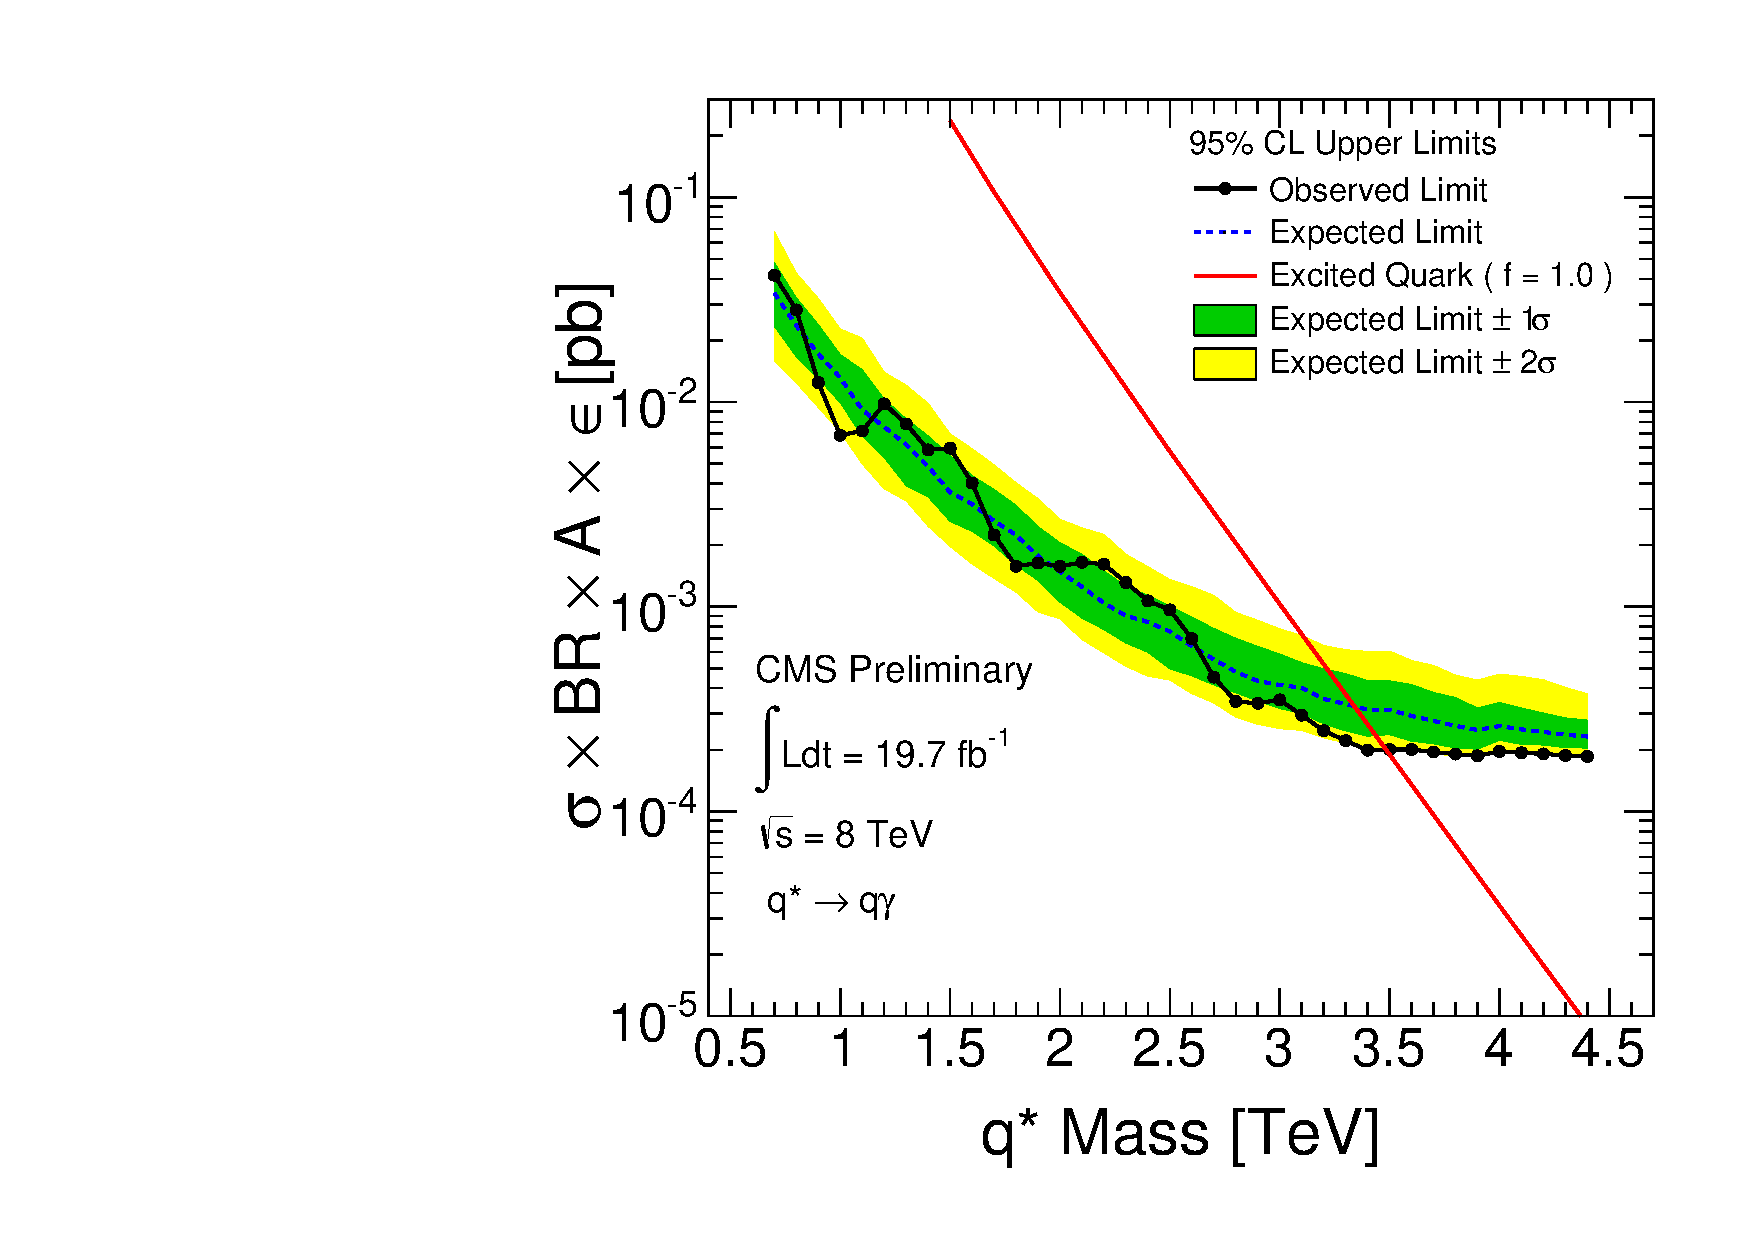
\includegraphics[width=10cm,height=8cm]{ch6/plots/ExcitedQuarksToGJ_f1p0_ObseExp_xsAccEff_Limits.pdf}
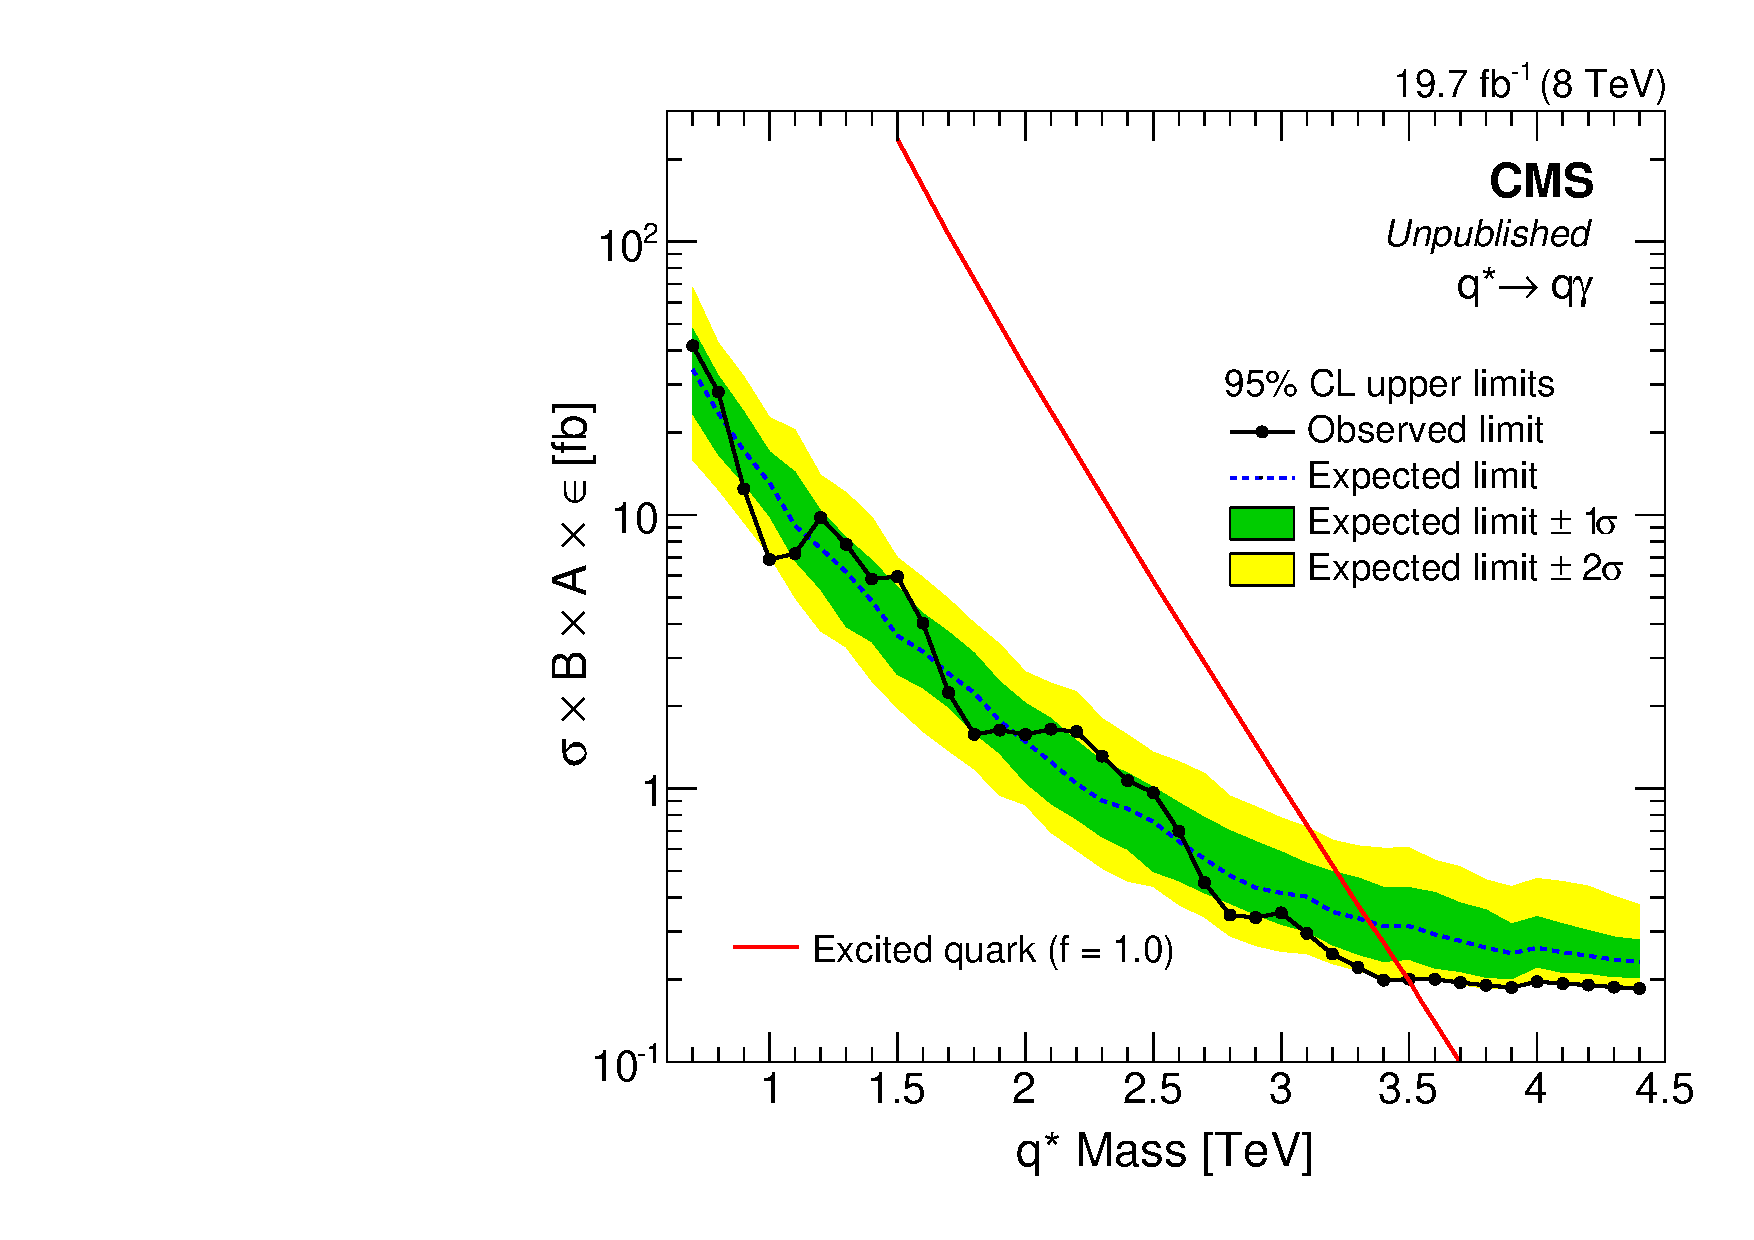
\includegraphics[width=10cm,height=8cm]{ch6/plots/ExcitedQuarksToGJ_f1p0_ObseExp_xsAccEff_Limits_fb.pdf}
 \caption{ The expected and observed 95\% CL upper limits on $\sigma\times\mathcal{B}\times{A}\times\epsilon$ for $\qstar\to\gamjet$ with coupling
           parameter $f=1.0$. The upper limits are also compared with theoretical prediction for \qstar production. The uncertainty at $1\sigma$ 
           and $2\sigma$ levels are shown as green and yellow bands, around the expected limit.}
\label{fig:qstarLimitfull}
\end{figure}
\begin{figure}[h!]
\centering
%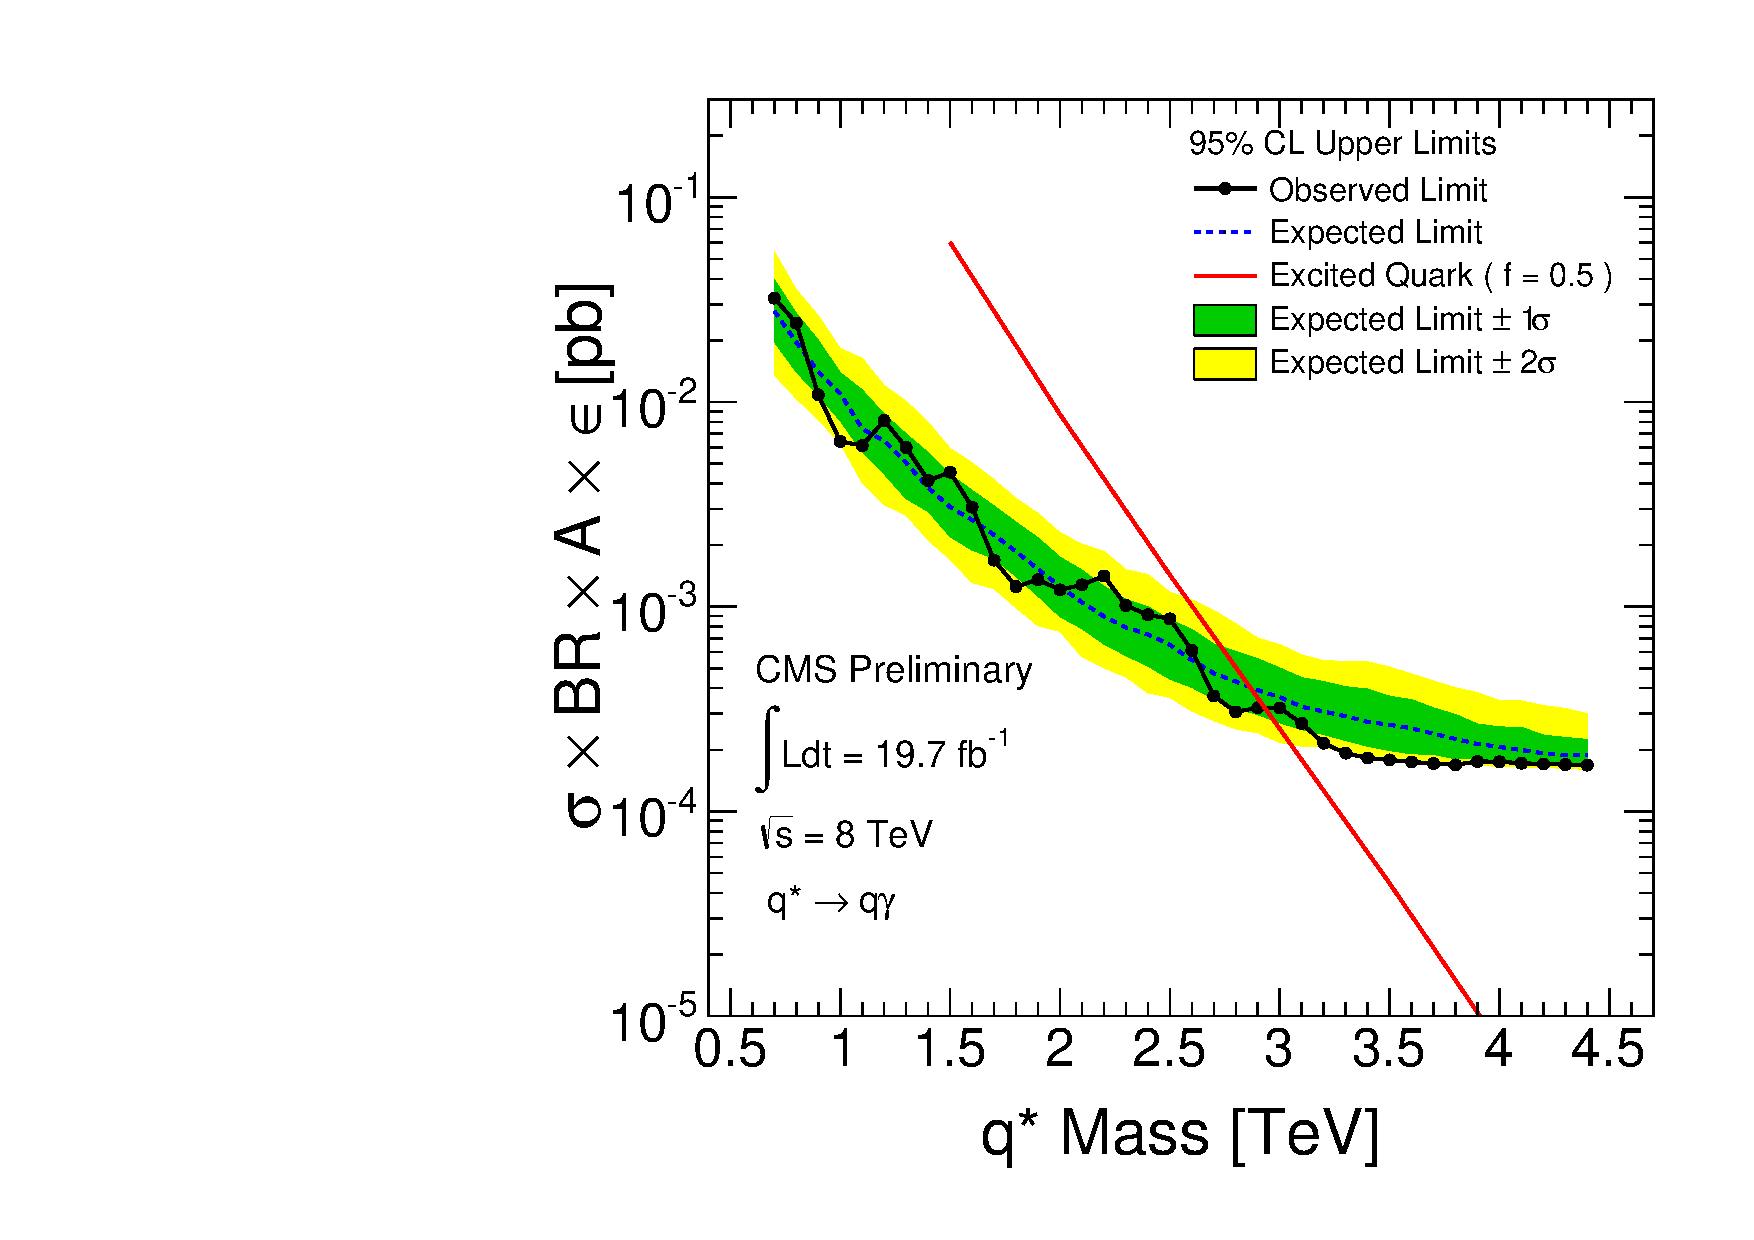
\includegraphics[width=10cm,height=8cm]{ch6/plots/ExcitedQuarksToGJ_f0p5_ObseExp_xsAccEff_Limits.pdf}
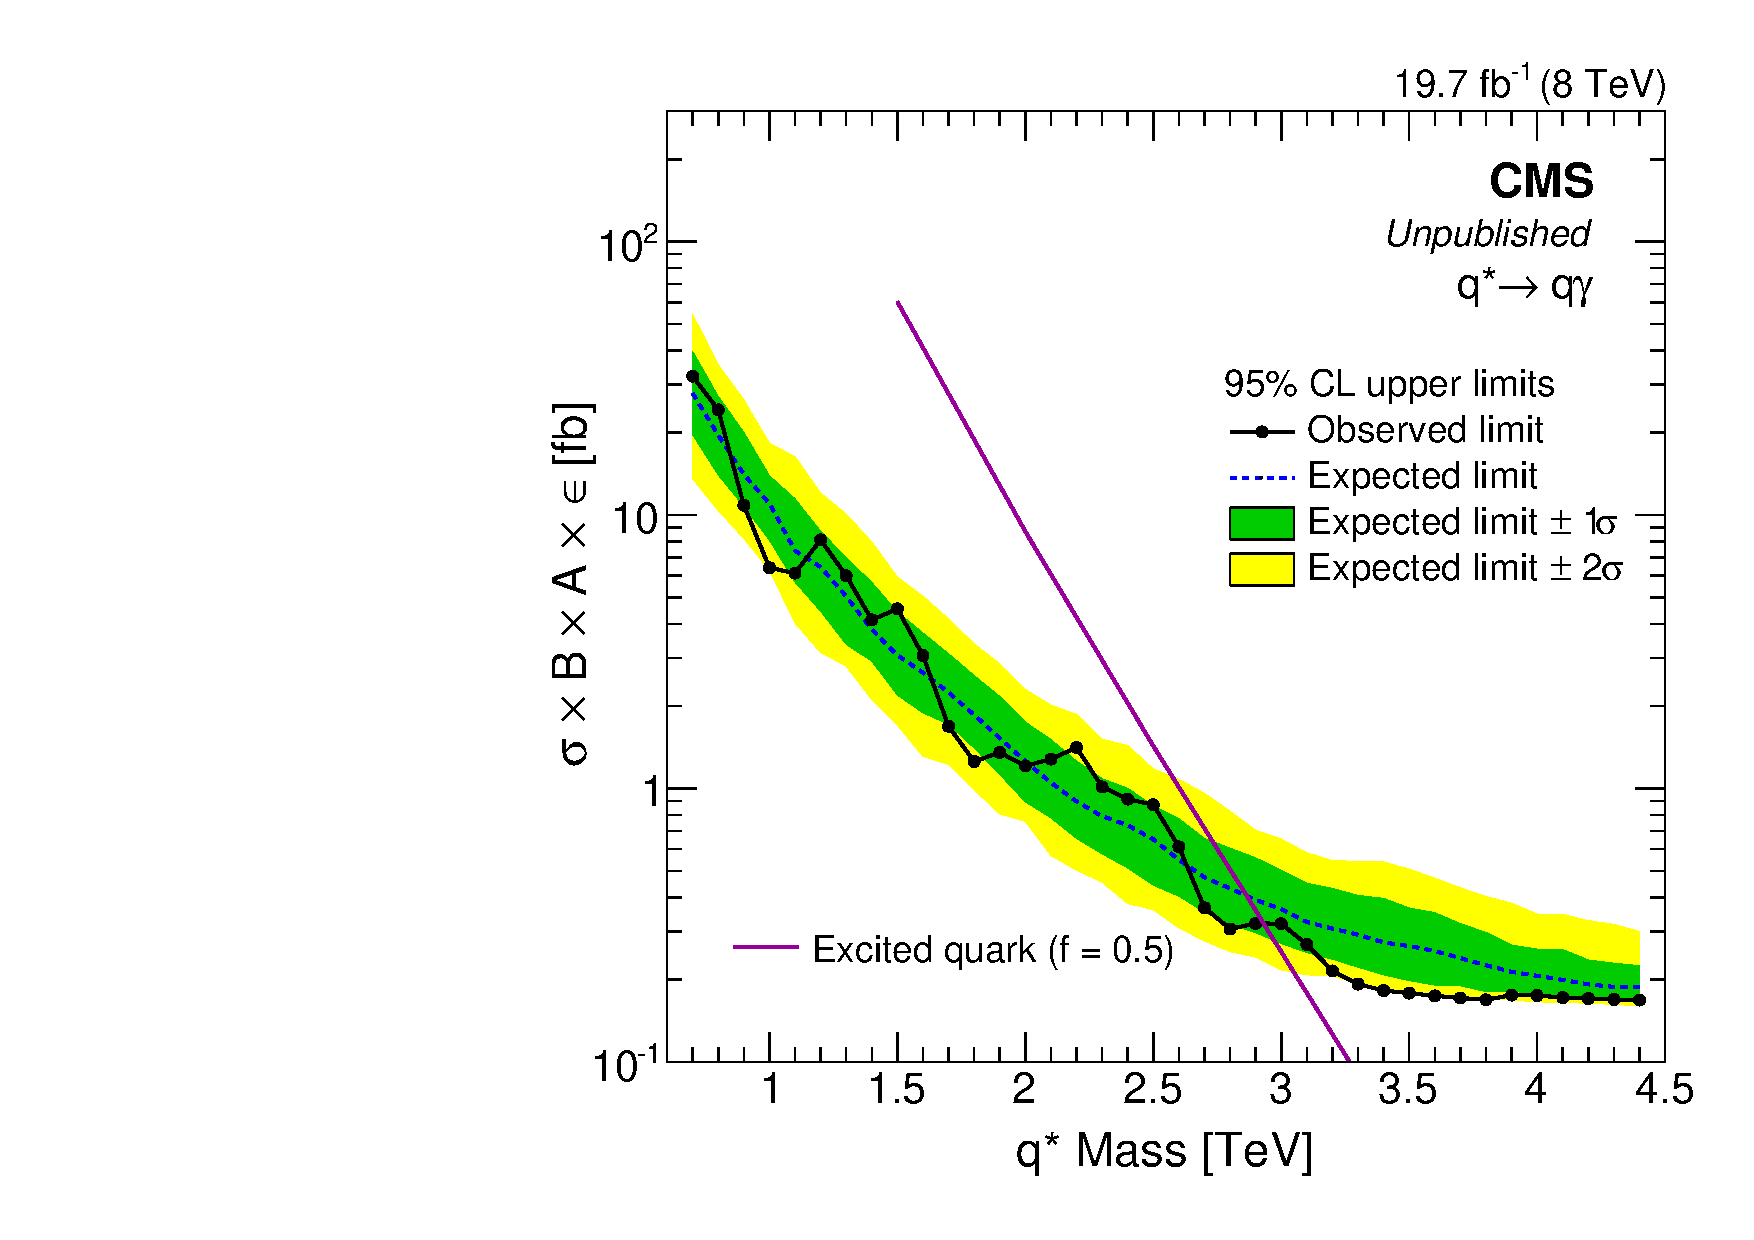
\includegraphics[width=10cm,height=8cm]{ch6/plots/ExcitedQuarksToGJ_f0p5_ObseExp_xsAccEff_Limits_fb.pdf}
 \caption{The expected and observed 95\% CL upper limits on $\sigma\times\mathcal{B}\times{A}\times\epsilon$ for $\qstar\to\gamjet$ with coupling
          parameter $f=0.5$. The upper limits are also compared with theoretical prediction for \qstar production. The uncertainty at $1\sigma$ 
          and $2\sigma$ levels are shown as green and yellow bands, around the expected limit.}
\label{fig:qstarLimithalf}
\end{figure}

\Figs{\ref{fig:qstarXSLimitfull}} and~\ref{fig:qstarXSLimithalf}, respectively, show the model independent limits on $\sigma\times\mathcal{B}$ for 
coupling multipliers, $f=1.0$ and $f=0.5$.
\begin{figure}[h!]
\centering
%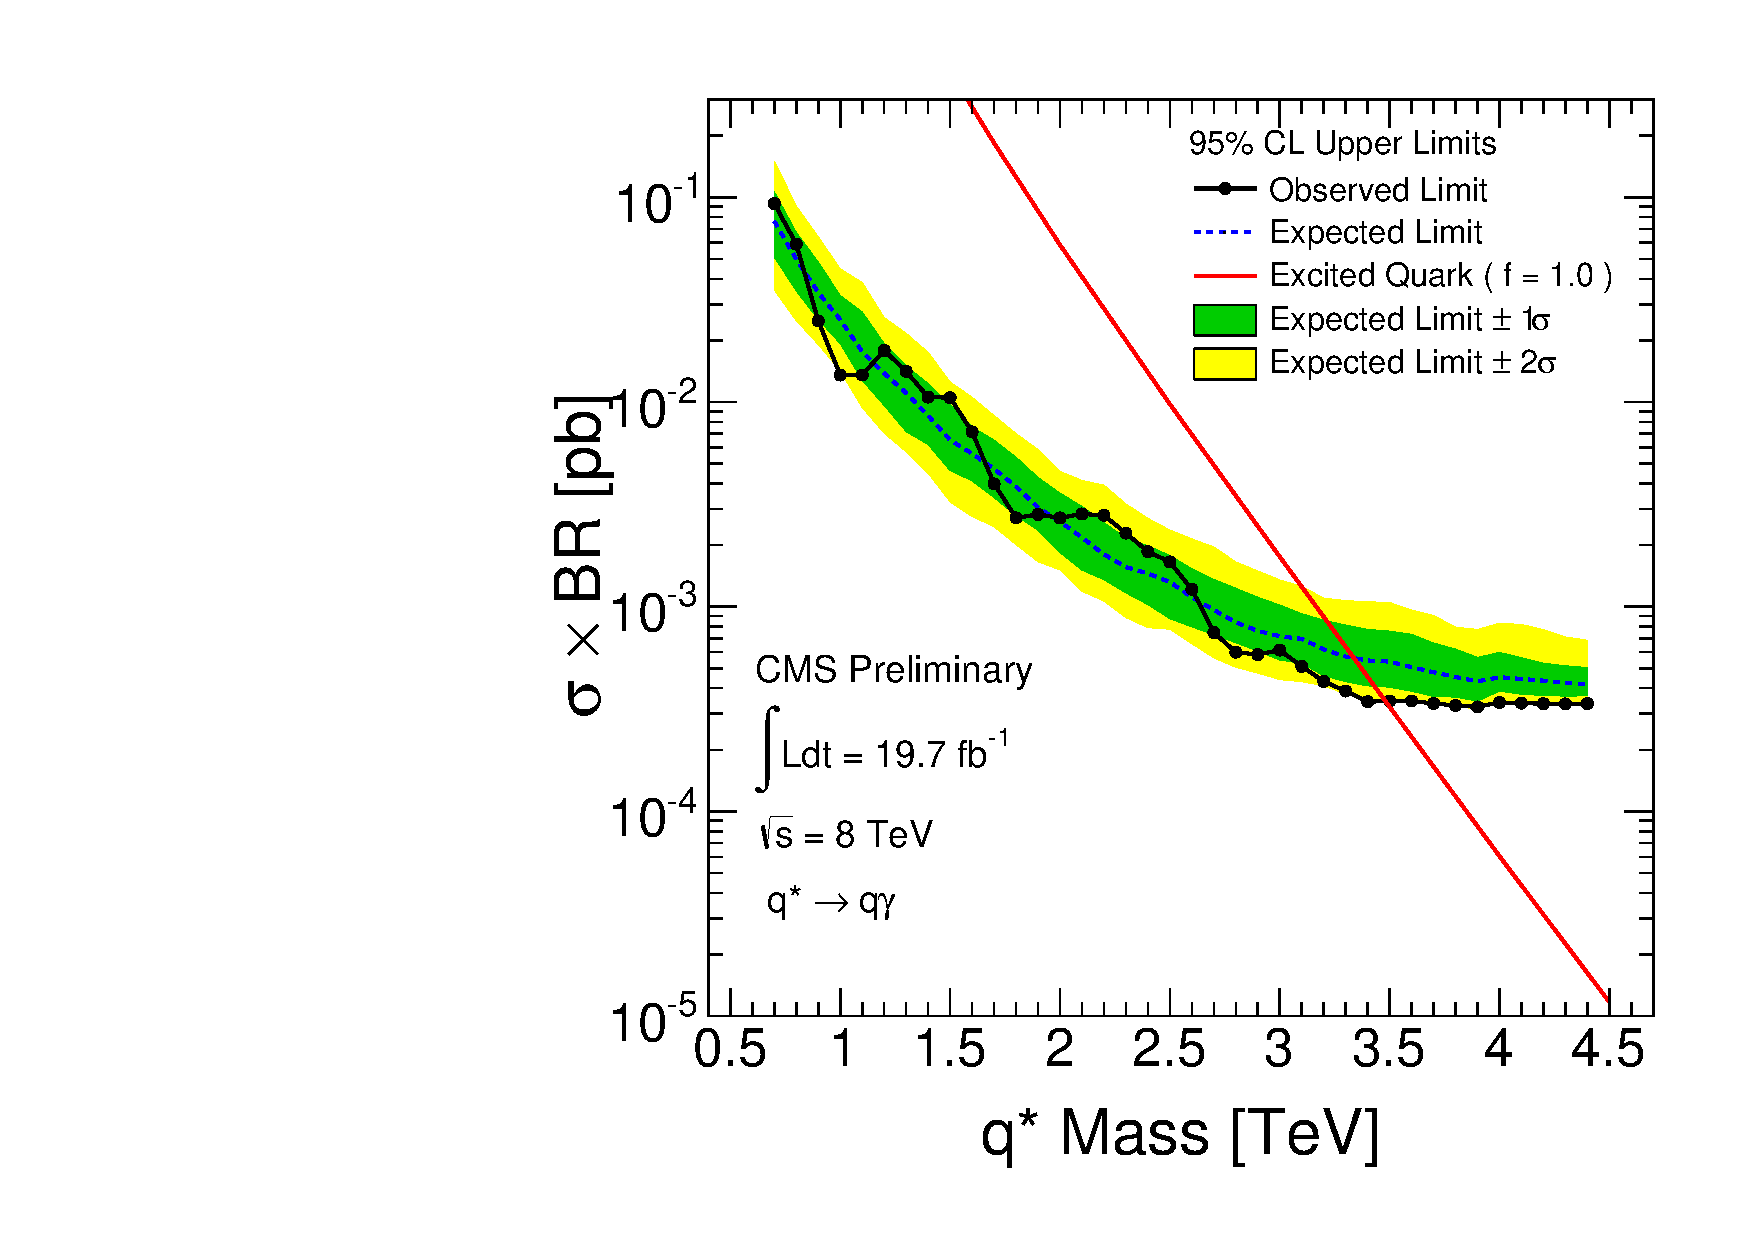
\includegraphics[width=10cm,height=8cm]{ch6/plots/ExcitedQuarksToGJ_f1p0_ObseExp_xs_Limits.pdf}
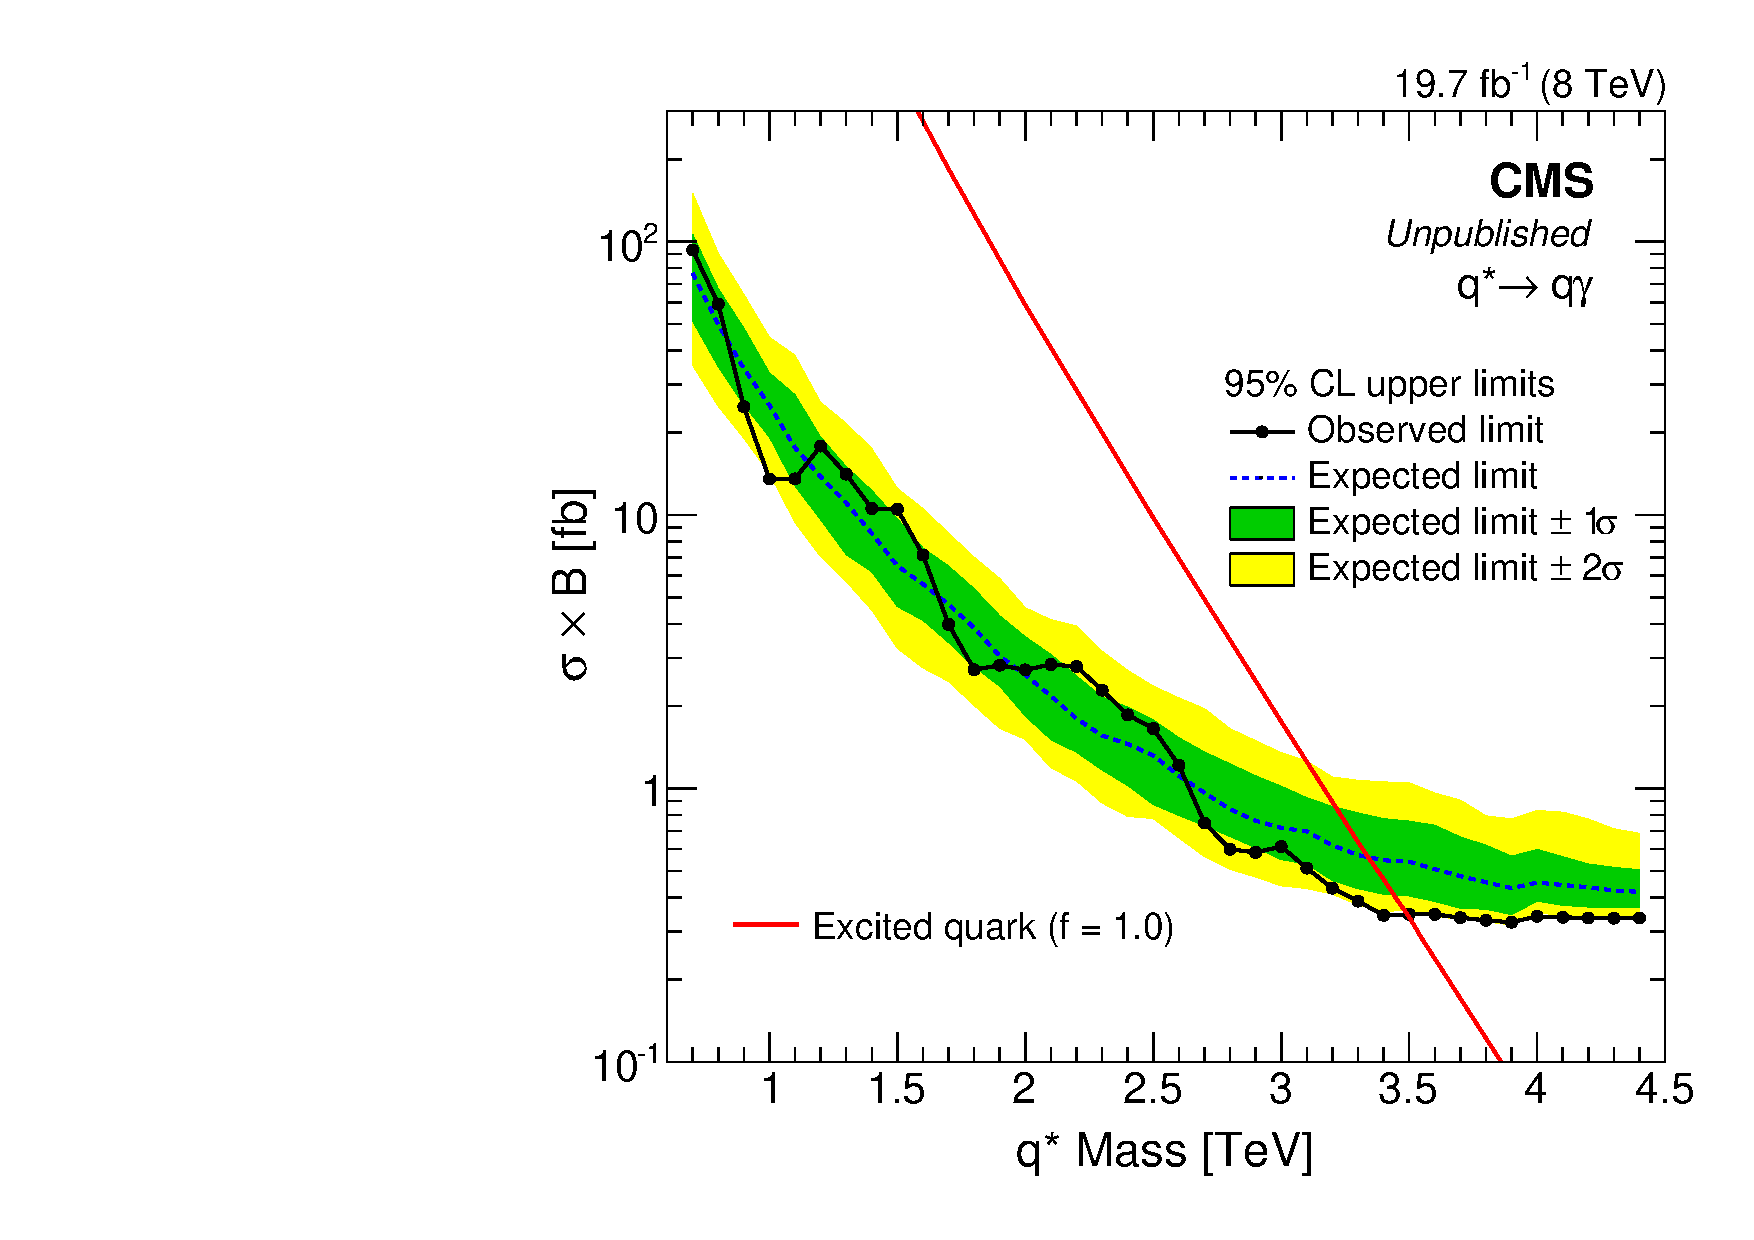
\includegraphics[width=10cm,height=8cm]{ch6/plots/ExcitedQuarksToGJ_f1p0_ObseExp_xs_Limits_fb.pdf}
 \caption{ The expected and observed 95\% CL upper limits on $\sigma\times\mathcal{B}$ for $\qstar\to\gamjet$ with coupling parameter $f=1.0$. The 
           upper limits are also compared with theoretical predictions for \qstar production. The uncertainty at $1\sigma$ and $2\sigma$ levels are
           shown as green and yellow bands, around the expected limit.}
\label{fig:qstarXSLimitfull}
\end{figure}
\begin{figure}[h!]
\centering
%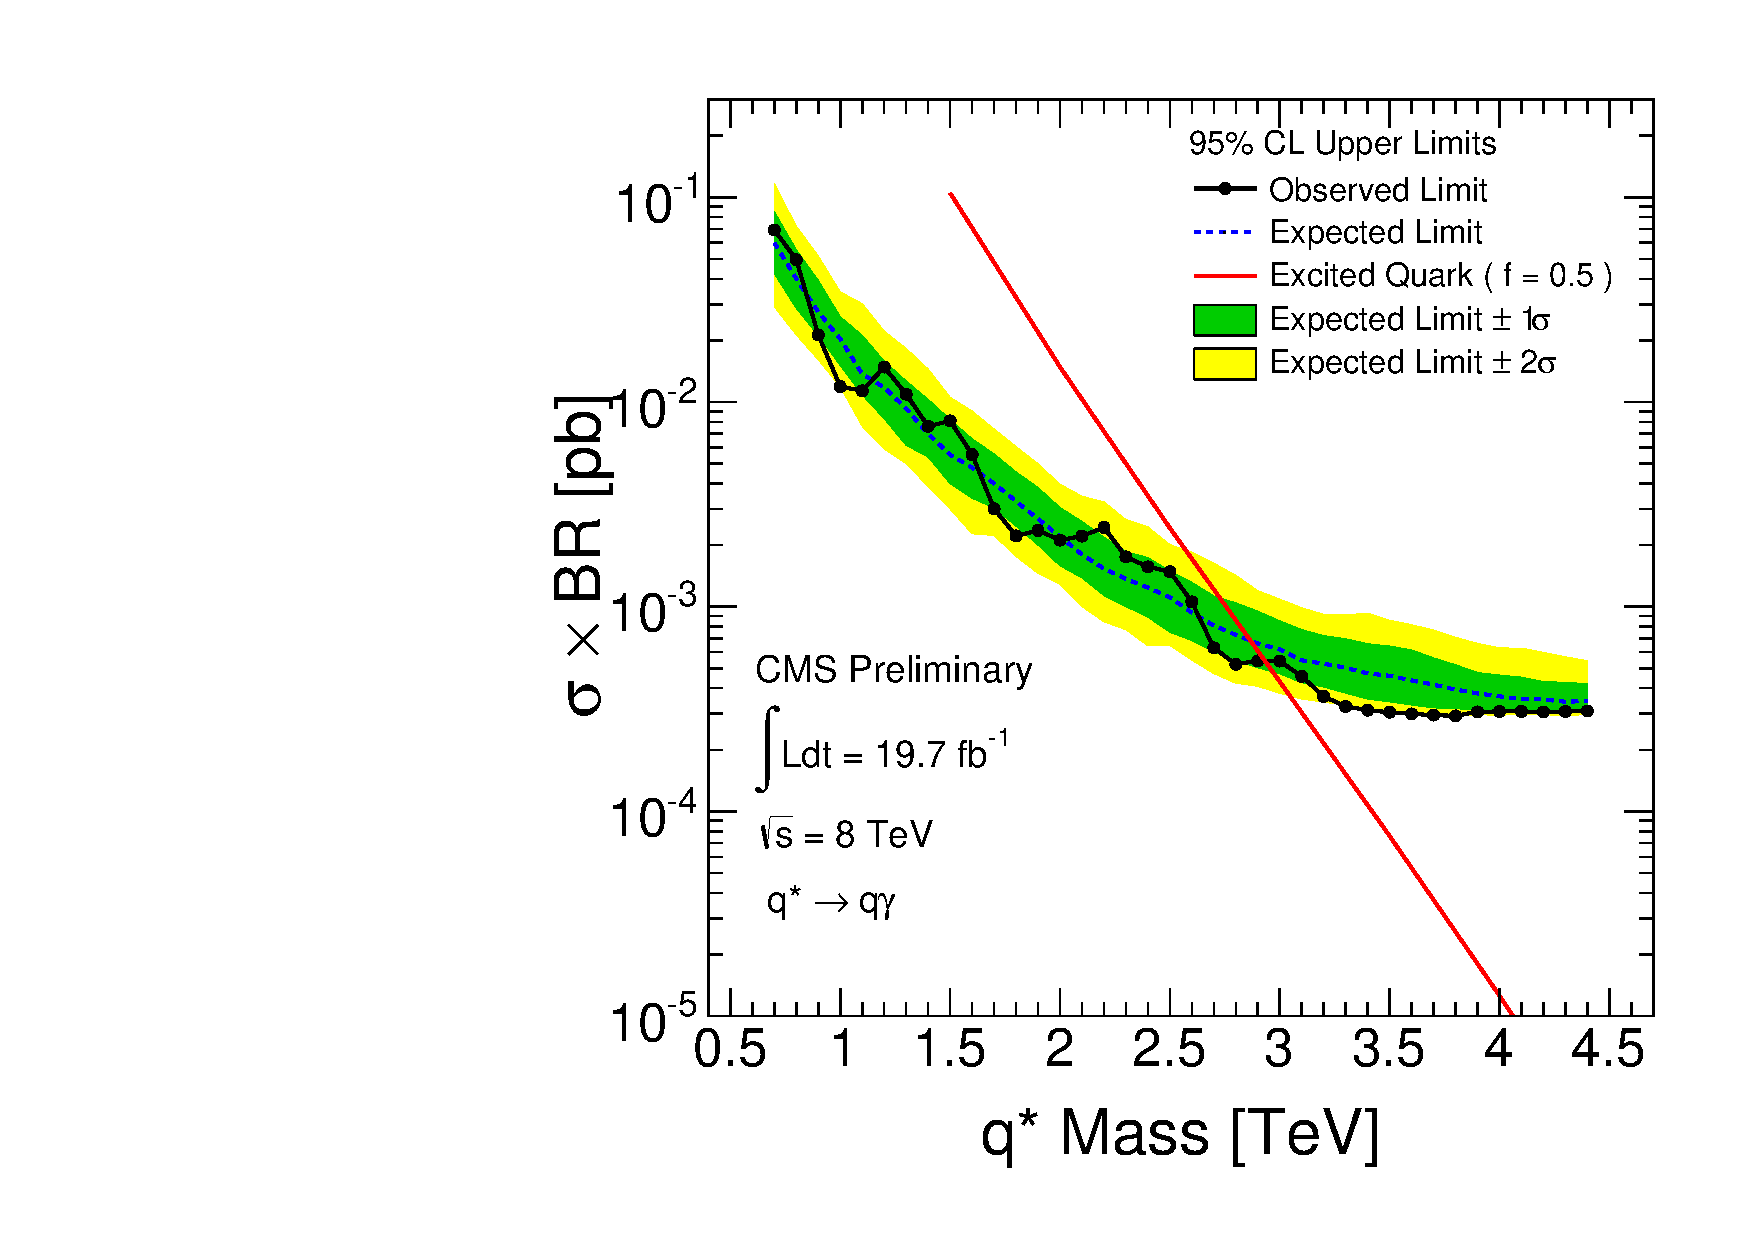
\includegraphics[width=10cm,height=8cm]{ch6/plots/ExcitedQuarksToGJ_f0p5_ObseExp_xs_Limits.pdf}
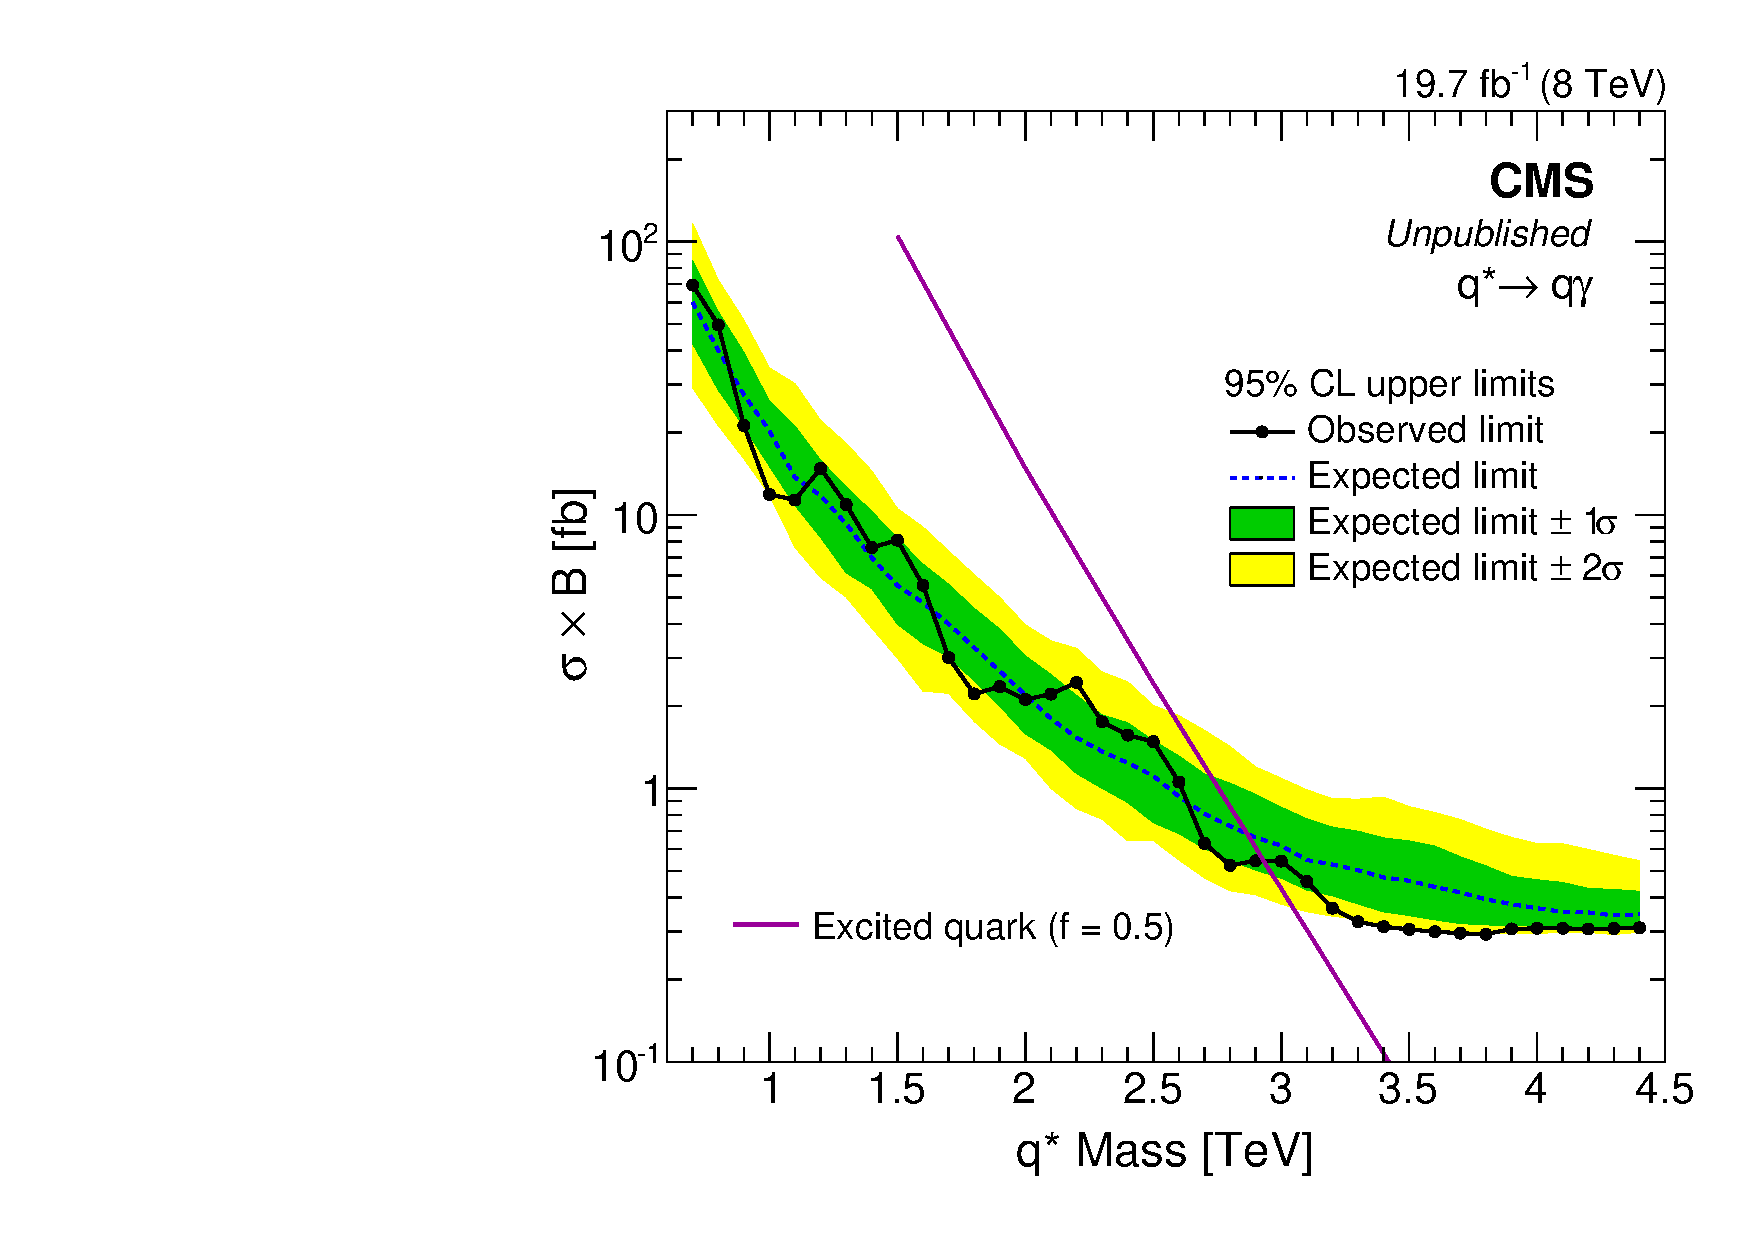
\includegraphics[width=10cm,height=8cm]{ch6/plots/ExcitedQuarksToGJ_f0p5_ObseExp_xs_Limits_fb.pdf}
 \caption{ The expected and observed 95\% CL upper limits on $\sigma\times\mathcal{B}$ for $\qstar\to\gamjet$ with coupling parameter $f=0.5$. The   
           upper limits are also compared with theoretical predictions for \qstar production. The uncertainty at $1\sigma$ and $2\sigma$ levels are 
           shown as green and yellow bands, around the expected limit.}
\label{fig:qstarXSLimithalf}
\end{figure}
For estimating these model independent limits on the cross section an additional systematics uncertainty of 4\% on correction factors and
statistical uncertainty on $A\times\epsilon$, was propagated in the limit setting procedure. The observed upper limits were compared to the 
leading order theoretical predictions to estimate the lower mass bounds on the excited quarks as shown in \figs{\ref{fig:qstarXSLimitfull}} 
and~\ref{fig:qstarXSLimithalf}. A lower bound of 3.5\unit{TeV} (2.9\unit{TeV}) on the mass of \qstar is set for coupling multipliers, 
$f=1.0$ $(0.5)$. The corresponding expected limits were found to be 3.4 (2.8)\unit{TeV}.

These cross section upper limits for coupling multiplier half the strength of standard couplings $f=1.0$, \ie, $f=0.5$ are the first set of results
from any LHC experiment at 8\unit{TeV}. The comparison of observed limits for $f=0.5$ and $f=1.0$ coupling scenarios has been shown in 
\fig{\ref{fig:compareLimit}}. Table~\ref{Table:ObsLimits} shows the comparison of expected and observed limits for couplings $f=0.5$ and $f=1.0$ in 
a tabular form. \Fig{\ref{fig:LimitsfullHalf}} shows the expected and observed 95\% CL upper limit on $\sigma\times\mathcal{B}$ for \qstar and a 
comparison with theoretical predictions for couplings $f=1.0$ and $f=0.5$ on the same canvas. If one takes into account the theoretical uncertainty 
on signal, the observed limit on \mqstar changes by $\pm$0.2\%. 
\begin{figure}[h!]
\centering
% 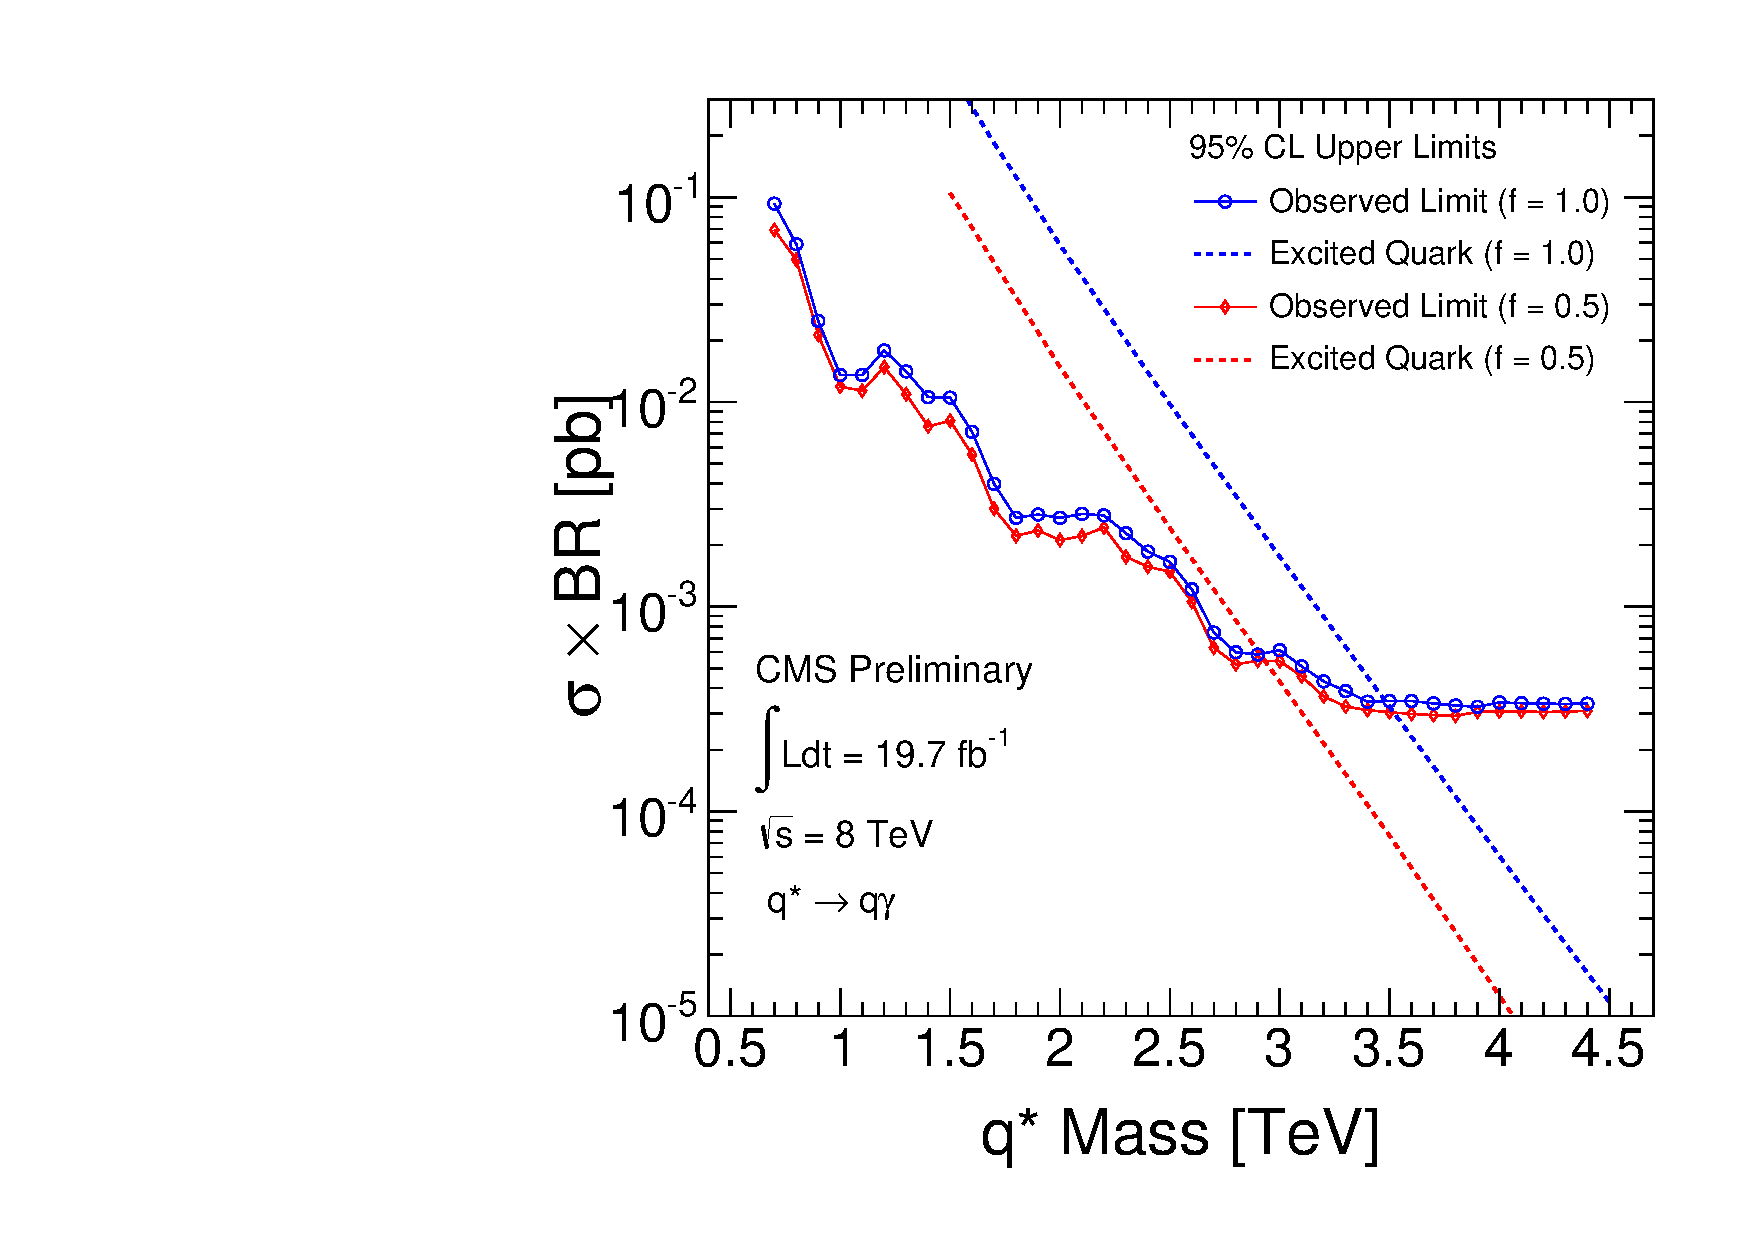
\includegraphics[width=10cm,height=8cm]{ch6/plots/ExcitedQuarksToGJ_Comparef0p5f1p0_ObseExp_xs_Limits.pdf}
 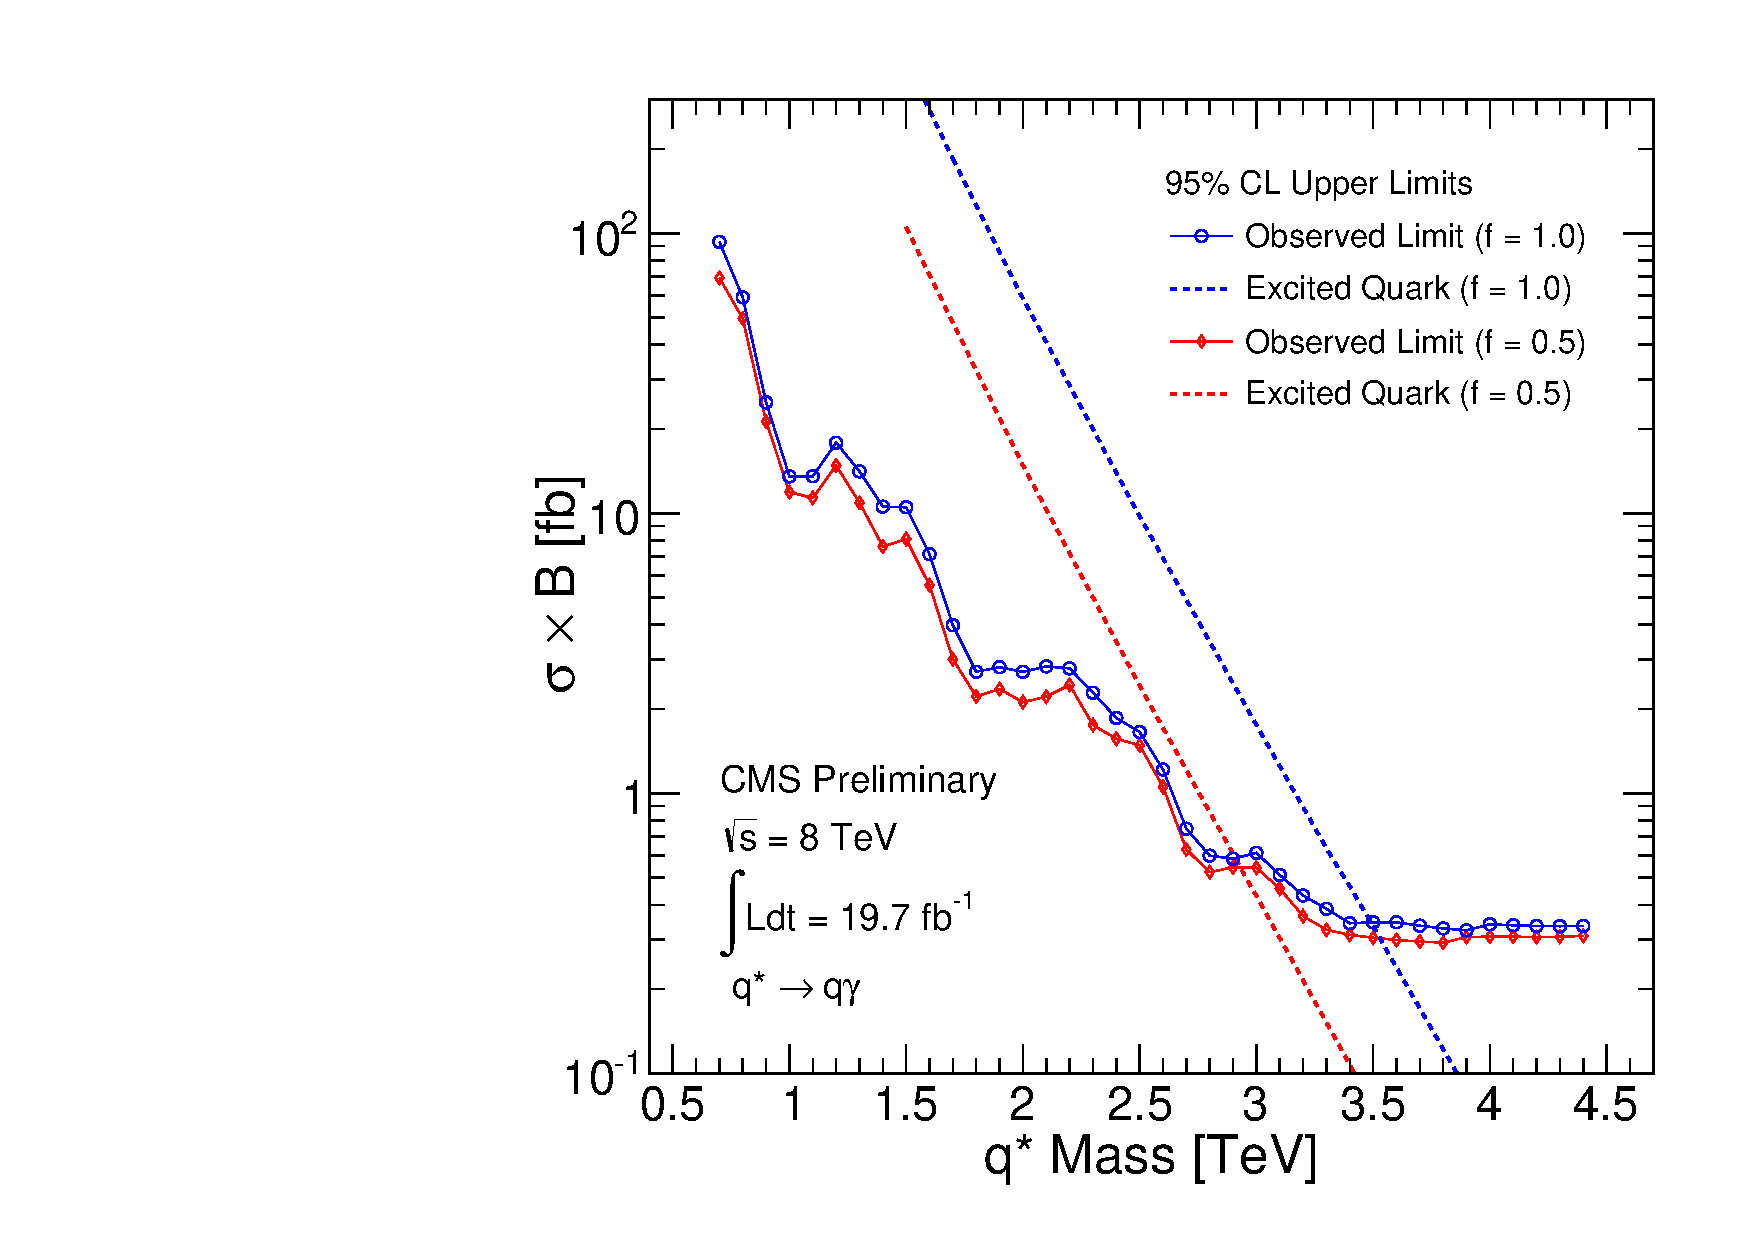
\includegraphics[width=10cm,height=8cm]{ch6/plots/ExcitedQuarksToGJ_Comparef0p5f1p0_ObseExp_xs_Limits_fb.pdf}
 \caption{Comparison of observed limits for excited quarks with $f=0.5$ and 1.0 respectively. }
\label{fig:compareLimit}
\end{figure}
\begin{table}[h!]
\begin{center}
\begin{tabular}{c||cc||cc}
\hline
Mass     & \multicolumn{2}{c||}{$f=0.5$} & \multicolumn{2}{c}{$f=1.0$} \\
(\unit{TeV}) & Expected  & Observed & Expected & Observed  \\
\hline
\hline
0.7 & 59.954  & 69.295 &  76.369 &  93.179 \\
0.8 & 40.079  & 49.590 &  49.836 &  59.039 \\
0.9 & 27.571  & 21.270 &  34.298 &  24.896 \\
1.0 & 20.329  & 11.904 &  25.235 &  13.543 \\
1.1 & 13.721  & 11.348 &  17.629 &  13.559 \\
1.2 & 11.776  & 14.815 &  13.806 &  17.872 \\
1.3 & 9.2835  & 10.919 &  11.073 &  14.112 \\
1.4 & 6.9799  & 7.6101 &  8.5730 &  10.564 \\
1.5 & 5.5258  & 8.0946 &  6.5187 &  10.508 \\
1.6 & 4.7815  & 5.5372 &  5.5947 &  7.1461 \\
1.7 & 3.9969  & 3.0119 &  4.7100 &  3.9834 \\
1.8 & 3.2762  & 2.2179 &  3.8666 &  2.7188 \\
1.9 & 2.6871  & 2.3577 &  3.0480 &  2.8226 \\
2.0 & 2.1982  & 2.1161 &  2.6015 &  2.7155 \\
2.1 & 1.8008  & 2.2140 &  2.1788 &  2.8401 \\
2.2 & 1.5338  & 2.4396 &  1.8017 &  2.7940 \\
2.3 & 1.3667  & 1.7533 &  1.5616 &  2.2873 \\
2.4 & 1.2400  & 1.5670 &  1.4529 &  1.8591 \\
2.5 & 1.1111  & 1.4838 &  1.3205 &  1.6559 \\
2.6 & 0.9361  & 1.0562 &  1.1133 &  1.2165 \\
2.7 & 0.8079  & 0.6300 &  0.9645 &  0.7477 \\
2.8 & 0.7286  & 0.5232 &  0.8387 &  0.5991 \\
2.9 & 0.6610  & 0.5442 &  0.7625 &  0.5839 \\
3.0 & 0.6179  & 0.5424 &  0.7173 &  0.6132 \\
3.1 & 0.5474  & 0.4566 &  0.6965 &  0.5111 \\
3.2 & 0.5271  & 0.3646 &  0.6197 &  0.4316 \\
3.3 & 0.5026  & 0.3255 &  0.5708 &  0.3871 \\
3.4 & 0.4729  & 0.3123 &  0.5463 &  0.3436 \\
3.5 & 0.4597  & 0.3051 &  0.5394 &  0.3462 \\
3.6 & 0.4365  & 0.2994 &  0.5071 &  0.3463 \\
3.7 & 0.4163  & 0.2956 &  0.4783 &  0.3369 \\
3.8 & 0.3933  & 0.2930 &  0.4537 &  0.3292 \\
3.9 & 0.3773  & 0.3065 &  0.4319 &  0.3241 \\
4.0 & 0.3648  & 0.3080 &  0.4527 &  0.3407 \\
4.1 & 0.3537  & 0.3081 &  0.4436 &  0.3378 \\
4.2 & 0.3522  & 0.3061 &  0.4352 &  0.3360 \\
4.3 & 0.3433  & 0.3075 &  0.4237 &  0.3353 \\
4.4 & 0.3464  & 0.3096 &  0.4187 &  0.3361 \\
\hline
\end{tabular}
\caption{Expected and observed 95\% CL upper limits on $\sigma\times\mathcal{B}$ (in fb) as a function of resonance mass for couplings strengths $f=0.5$ and 1.0 respectively.}
   \label{Table:ObsLimits}
\end{center}
\end{table}

%\begin{table}[h!]
\begin{center}
\begin{tabular}{c||cc||cc}
\hline
Mass     & \multicolumn{2}{c}{Expected} & \multicolumn{2}{c}{Observed} \\
(\unit{TeV}) & $f=0.5$  & $f=1.0$ & $f=0.5$ & $f=1.0$  \\
\hline
\hline
0.7 & 59.954  &  76.369 & 69.295 &  93.179 \\
0.8 & 40.079  &  49.836 & 49.590 &  59.039 \\
0.9 & 27.571  &  34.298 & 21.270 &  24.896 \\
1.0 & 20.329  &  25.235 & 11.904 &  13.543 \\
1.1 & 13.721  &  17.629 & 11.348 &  13.559 \\
1.2 & 11.776  &  13.806 & 14.815 &  17.872 \\
1.3 & 9.2835  &  11.073 & 10.919 &  14.112 \\
1.4 & 6.9799  &  8.5730 & 7.6101 &  10.564 \\
1.5 & 5.5258  &  6.5187 & 8.0946 &  10.508 \\
1.6 & 4.7815  &  5.5947 & 5.5372 &  7.1461 \\
1.7 & 3.9969  &  4.7100 & 3.0119 &  3.9834 \\
1.8 & 3.2762  &  3.8666 & 2.2179 &  2.7188 \\
1.9 & 2.6871  &  3.0480 & 2.3577 &  2.8226 \\
2.0 & 2.1982  &  2.6015 & 2.1161 &  2.7155 \\
2.1 & 1.8008  &  2.1788 & 2.2140 &  2.8401 \\
2.2 & 1.5338  &  1.8017 & 2.4396 &  2.7940 \\
2.3 & 1.3667  &  1.5616 & 1.7533 &  2.2873 \\
2.4 & 1.2400  &  1.4529 & 1.5670 &  1.8591 \\
2.5 & 1.1111  &  1.3205 & 1.4838 &  1.6559 \\
2.6 & 0.9361  &  1.1133 & 1.0562 &  1.2165 \\
2.7 & 0.8079  &  0.9645 & 0.6300 &  0.7477 \\
2.8 & 0.7286  &  0.8387 & 0.5232 &  0.5991 \\
2.9 & 0.6610  &  0.7625 & 0.5442 &  0.5839 \\
3.0 & 0.6179  &  0.7173 & 0.5424 &  0.6132 \\
3.1 & 0.5474  &  0.6965 & 0.4566 &  0.5111 \\
3.2 & 0.5271  &  0.6197 & 0.3646 &  0.4316 \\
3.3 & 0.5026  &  0.5708 & 0.3255 &  0.3871 \\
3.4 & 0.4729  &  0.5463 & 0.3123 &  0.3436 \\
3.5 & 0.4597  &  0.5394 & 0.3051 &  0.3462 \\
3.6 & 0.4365  &  0.5071 & 0.2994 &  0.3463 \\
3.7 & 0.4163  &  0.4783 & 0.2956 &  0.3369 \\
3.8 & 0.3933  &  0.4537 & 0.2930 &  0.3292 \\
3.9 & 0.3773  &  0.4319 & 0.3065 &  0.3241 \\
4.0 & 0.3648  &  0.4527 & 0.3080 &  0.3407 \\
4.1 & 0.3537  &  0.4436 & 0.3081 &  0.3378 \\
4.2 & 0.3522  &  0.4352 & 0.3061 &  0.3360 \\
4.3 & 0.3433  &  0.4237 & 0.3075 &  0.3353 \\
4.4 & 0.3464  &  0.4187 & 0.3096 &  0.3361 \\
\hline
\end{tabular}
\caption{Expected and observed 95\% CL upper limits on $\sigma\times\mathcal{B}$ as a function of resonance mass for couplings strengths $f=0.5$ and $f=1.0$.}
   \label{Table:ObsLimits}
\end{center}
\end{table}

%\begin{table}[h!]
\centering
\begin{tabular}{rcc|rcc}
\hline
Mass    & \multicolumn{2}{c}{Upper limit (fb)} &  Mass  & \multicolumn{2}{c}{Upper limit (fb)} \\
(\unit{TeV})   & Expected & Observed & (\unit{TeV}) & Expected & Observed \\ 
\hline
0.7  &  76.4 &  93.2 & 2.6 &  1.11 &  1.22 \\
0.8  &  49.8 &  59.0 & 2.7 &  0.96 &  0.75 \\
0.9  &  34.3 &  24.9 & 2.8 &  0.84 &  0.60 \\
1.0 &  25.2 &  13.5 & 2.9 &  0.76 &  0.58 \\
1.1 &  17.6 &  13.6 & 3.0 &  0.72 &  0.61 \\
1.2 &  13.8 &  17.9 & 3.1 &  0.70 &  0.51 \\
1.3 &  11.1 &  14.1 & 3.2 &  0.62 &  0.43 \\
1.4 &   8.57 &  10.6 & 3.3 &  0.57 &  0.39 \\
1.5 &   6.52 &  10.5 & 3.4 &  0.55 &  0.34 \\
1.6 &   5.59 &   7.15 & 3.5 &  0.54 &  0.35 \\
1.7 &   4.71 &   3.98 & 3.6 &  0.51 &  0.35 \\
1.8 &   3.87 &   2.72 & 3.7 &  0.48 &  0.34 \\
1.9 &   3.05 &   2.82 & 3.8 &  0.45 &  0.33 \\
2.0 &   2.60 &   2.72 & 3.9 &  0.43 &  0.32 \\
2.1 &   2.18 &   2.84 & 4.0 &  0.45 &  0.34 \\
2.2 &   1.80 &   2.79 & 4.1 &  0.44 &  0.34 \\
2.3 &   1.56 &   2.29 & 4.2 &  0.44 &  0.34 \\
2.4 &   1.45 &   1.86 & 4.3 &  0.42 &  0.34 \\
2.5 &   1.32 &   1.66 & 4.4 &  0.42 &  0.34 \\
\hline
\end{tabular}
%  \caption{The expected and observed 95\% CL upper limits on $\sigma\times\mathcal{B}$ for the production of excited quarks in the \gamjet final state, asssuming a coupling strength $f=1.0$.}
  \caption{The expected and observed 95\% CL upper limits on $\sigma\times\mathcal{B}$ for the production of excited quarks in the \gamjet final state, asssuming a coupling strength $f=1.0$.}
   \label{Table:ObsLimits}
\end{table}



As the observed width of \qstar resonance is dominated by the experimental resolution, the dependence of $\sigma\times\mathcal{B}$ cross section
upper limit on $f$ was found to be negligible for $f\le1$. Using the theoretical predictions, cross sections were evaluated for various \qstar mass
 points for different couplings ranging from $f=1.0$ to as low as $f=0.04$ as reported in~\tab{\ref{Table:AllfXS}}. These theoretical predictions 
were then used to exclude the mass of excited quarks for respective set of coupling strength as shown in \fig{\ref{fig:LimitAllCouplings}}.
%%---------------TABLE FOR MC samples-------------------
\begin{table}[h!]
\begin{center}
%\begin{ruledtabular} 
\resizebox{16cm}{!}{
\begin{tabular}{|l|c|c|c|c|c|c|c|c|c|c|c|c|c|}
\hline
{\bf Mass (GeV) } & {\bf 0.04} & {\bf 0.05 } & {\bf 0.07 } & {\bf 0.1 } & {\bf 0.2 } & {\bf 0.3 } & {\bf 0.4 } & {\bf 0.5 } & {\bf 0.6 } & {\bf 0.7 } & {\bf 0.8 } & {\bf 0.9 } & {\bf 1.0 } \\
\hline
 700 & 3.962e-2  &  6.219e-2  &  1.217e-1  &  -  &  -  &  -  &  -  &  -  &  -  &  -  &  -  &  -  &  -  \\ 
 1000 & 6.859e-3  &  1.078e-2  &  2.102e-2  &  4.268e-2  &  1.707e-1  &  3.863e-1  &  6.838e-1  &  1.061e-0  &  1.541e-0  &  2.088e-0  &  2.695e-0  &  3.388e-0  &  4.177e-0  \\
 1500 & 6.743e-4  &  1.047e-3  &  2.074e-3  &  4.222e-3  &  1.699e-2  &  3.782e-2  &  6.692e-2  &  1.047e-1  &  1.507e-1  &  2.050e-1  &  2.653e-1  &  3.364e-1  &  4.121e-1  \\
 2000 &  5.918e-10  &  5.966e-8  & 5.890e-6   &  5.940e-4  &  2.377e-3  &  5.298e-3  &  9.497e-3  &  1.481e-2  &  2.129e-2  &  2.897e-2  &  3.751e-2  &  4.736e-2  &  5.830e-2  \\
 2500 &  -  &  -  &  -  &  9.721e-5  &  3.921e-4  &  8.754e-4  &  1.546e-3  &  2.436e-3  &  3.522e-3  &  4.756e-3  &  6.212e-3  &  7.898e-3  &  9.718e-3  \\
 3000 &  -  &  -  &  -  &  1.700e-5  &  6.831e-5  &  1.547e-4  &  2.738e-4  &  4.298e-4  &  6.233e-4  &  8.479e-4  &  1.111e-3  &  1.404e-3  &  1.761e-3  \\
 3500 &  -  &  -  &  -  &  2.989e-6  &  1.189e-5  &  2.657e-5  &  4.784e-5  &  7.575e-5  &  1.101e-4  &  1.512e-4  &  2.009e-4  &  2.601e-4  &  3.245e-4  \\
 4000 &  -  &  -  &  -  &  4.841e-7  &  1.950e-6  &  4.389e-6  &  7.837e-6  &  1.258e-5  &  1.882e-5  &  2.659e-5  &  3.602e-5  &  4.727e-5  &  6.041e-5  \\
 4500 &  -  &  -  &  -  &  7.163e-8  &  2.839e-7  &  6.518e-7  &  1.180e-6  &  1.928e-6  &  3.023e-6  &  4.574e-6  &  6.422e-6  &  8.772e-6  &  1.174e-5  \\
\hline
\end{tabular}
}
\caption{Cross section (in pb) of qstar signal samples for different couplings ($f=$ 0.04 to 1.0).}
%\end{ruledtabular}
   \label{Table:AllfXS}
\end{center}
\end{table}

%---------------TABLE FOR MC samples-------------------
\begin{table}[h!]
\begin{center}
%\begin{ruledtabular} 
\resizebox{16cm}{!}{
\begin{tabular}{|c|c|c|c|c|c|c|c|c|c|c|}
\hline

{\bf Couplings } &  \multicolumn{9}{c|}{\bf Mass (in GeV)} \\
\cline{2-10}
{$f$} & {\bf 700} & {\bf 1000 } & {\bf 1500 } & {\bf 2000 } & {\bf 2500 } & {\bf 3000 } & {\bf 3500 } & {\bf 4000 } & {\bf 4500 } \\
\hline
{\bf 0.04}  & 3.962e-2  & 6.859e-3  & 6.743e-4  & 5.918e-10 &     -     &     -     &     -     &     -     &     -     \\
{\bf 0.05 } & 6.219e-2  & 1.078e-2  & 1.047e-3  & 5.966e-8  &     -     &     -     &     -     &     -     &     -     \\
{\bf 0.07 } & 1.217e-1  & 2.102e-2  & 2.074e-3  & 5.890e-6  &     -     &     -     &     -     &     -     &     -     \\
{\bf 0.1 }  &    -      & 4.268e-2  & 4.222e-3  & 5.940e-4  & 9.721e-5  & 1.700e-5  & 2.989e-6  & 4.841e-7  & 7.163e-8  \\
{\bf 0.2 }  &    -      & 1.707e-1  & 1.699e-2  & 2.377e-3  & 3.921e-4  & 6.831e-5  & 1.189e-5  & 1.950e-6  & 2.839e-7  \\
{\bf 0.3 }  &    -      & 3.863e-1  & 3.782e-2  & 5.298e-3  & 8.754e-4  & 1.547e-4  & 2.657e-5  & 4.389e-6  & 6.518e-7  \\
{\bf 0.4 }  &    -      & 6.838e-1  & 6.692e-2  & 9.497e-3  & 1.546e-3  & 2.738e-4  & 4.784e-5  & 7.837e-6  & 1.180e-6  \\
{\bf 0.5 }  &    -      & 1.061e-0  & 1.047e-1  & 1.481e-2  & 2.436e-3  & 4.298e-4  & 7.575e-5  & 1.258e-5  & 1.928e-6  \\
{\bf 0.6 }  &    -      & 1.541e-0  & 1.507e-1  & 2.129e-2  & 3.522e-3  & 6.233e-4  & 1.101e-4  & 1.882e-5  & 3.023e-6  \\
{\bf 0.7 }  &    -      & 2.088e-0  & 2.050e-1  & 2.897e-2  & 4.756e-3  & 8.479e-4  & 1.512e-4  & 2.659e-5  & 4.574e-6  \\
{\bf 0.8 }  &    -      & 2.695e-0  & 2.653e-1  & 3.751e-2  & 6.212e-3  & 1.111e-3  & 2.009e-4  & 3.602e-5  & 6.422e-6  \\
{\bf 0.9 }  &    -      & 3.388e-0  & 3.364e-1  & 4.736e-2  & 7.898e-3  & 1.404e-3  & 2.601e-4  & 4.727e-5  & 8.772e-6  \\
{\bf 1.0 }  &    -      & 4.177e-0  & 4.121e-1  & 5.830e-2  & 9.718e-3  & 1.761e-3  & 3.245e-4  & 6.041e-5  & 1.174e-5  \\
\hline
\end{tabular}
}
\caption{Cross section (in pb) of \qstar signal samples for different couplings ($f=$ 0.04 to 1.0).}
%\end{ruledtabular}
   \label{Table:AllfXS}
\end{center}
\end{table}


Based on the lower mass limit for different set of coupling strengths as reported in \fig{\ref{fig:LimitAllCouplings}}, a mass region is excluded 
as a function of coupling parameter $f$ and is shown in \fig{\ref{fig:LimitMassCoupling}}. The results depicted in \fig{\ref{fig:LimitMassCoupling}} 
may also be used to present the limits on the excited quark mass, \mqstar, as a function of compositeness scale, $\Lambda$, if the assumption
$\Lambda=\mqstar$ is relaxed. This is justified as variation in $f$ and in $\mqstar/\Lambda$ also result in similar effect on the \qstar cross 
section. For example, if we assume $\Lambda=10\,\mqstar$ and standard model couplings, then using \fig{\ref{fig:LimitMassCoupling}} we exclude
excited quarks with mass $0.7<\mqstar<1.2\unit{TeV}$.
\begin{figure}[h!]
\centering
% 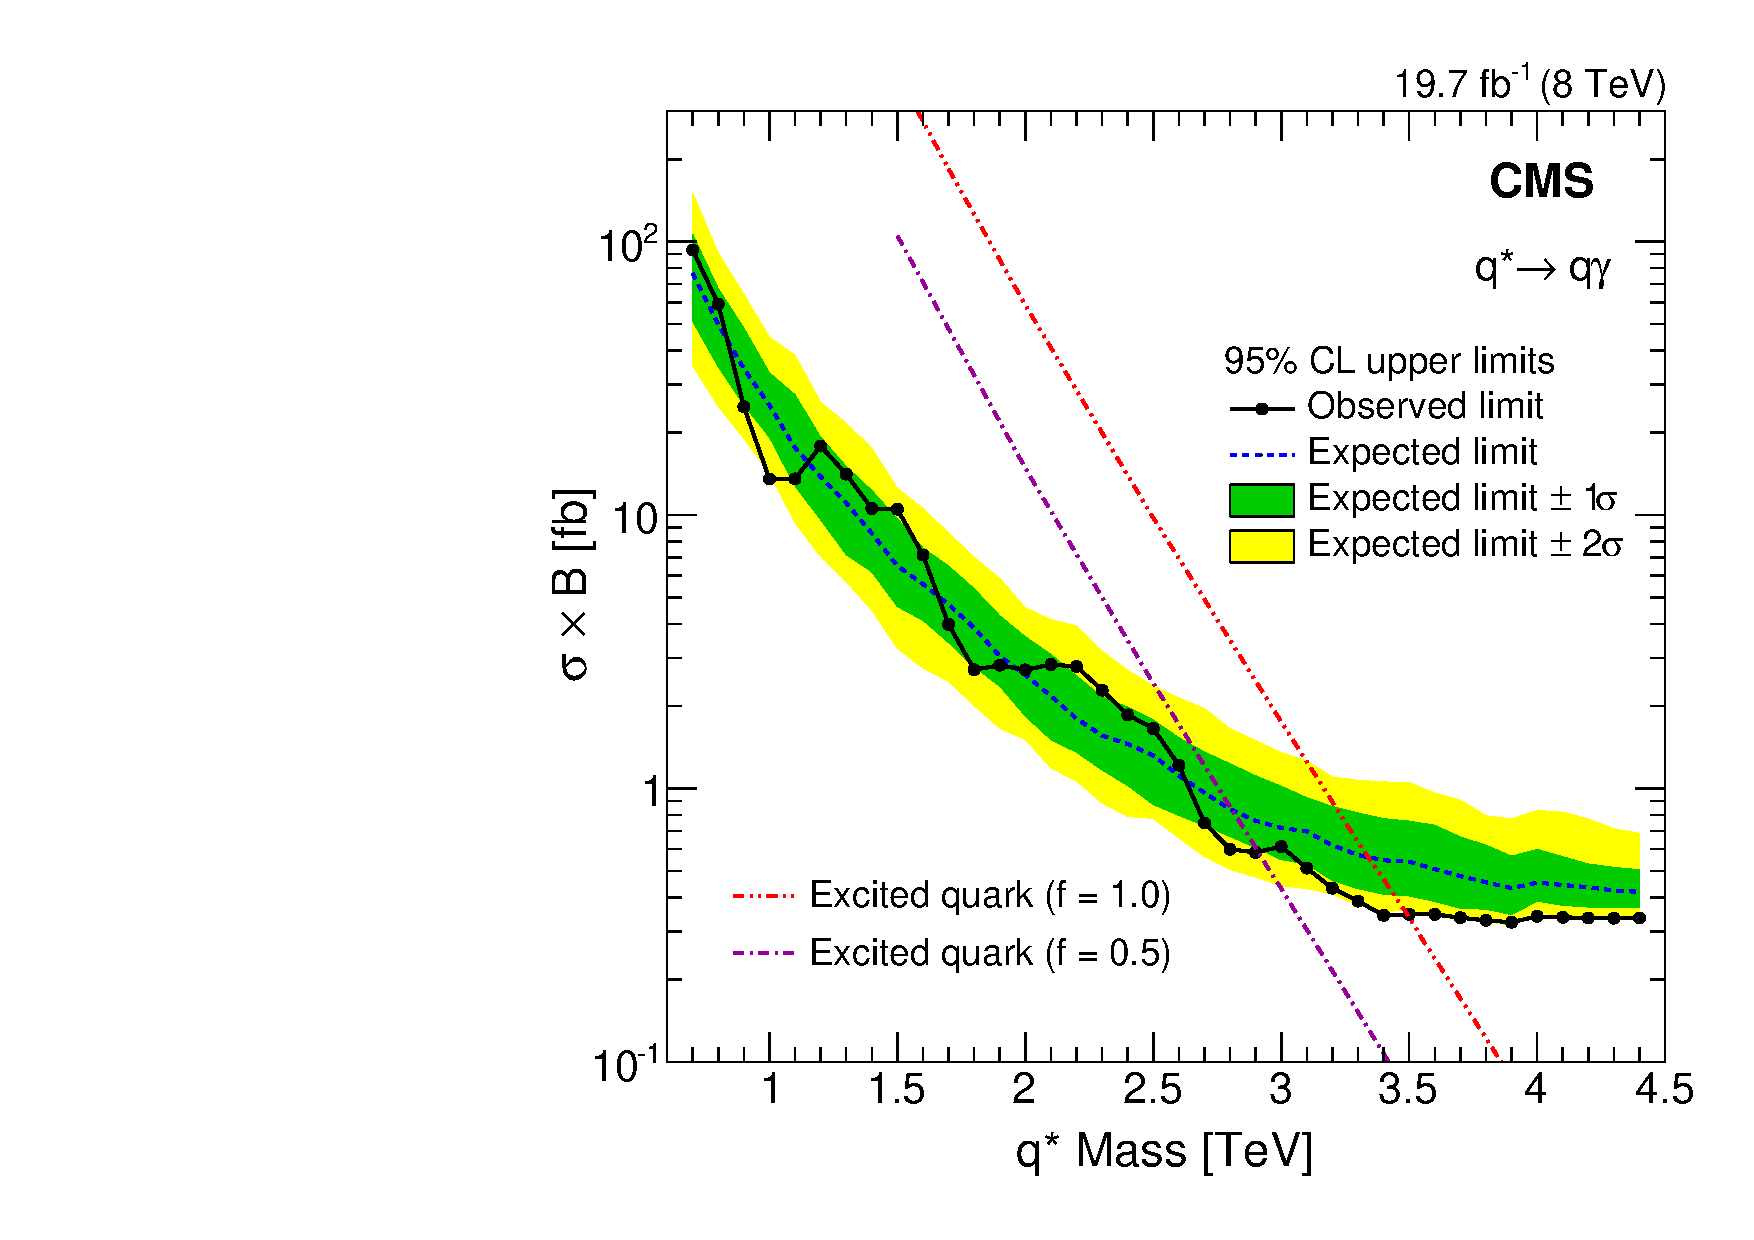
\includegraphics[width=10cm,height=8.5cm]{ch6/plots/ExcitedQuarksToGJ_fullfhalf_ObseExp_xs_Limits_paper_fb_v2.pdf}
 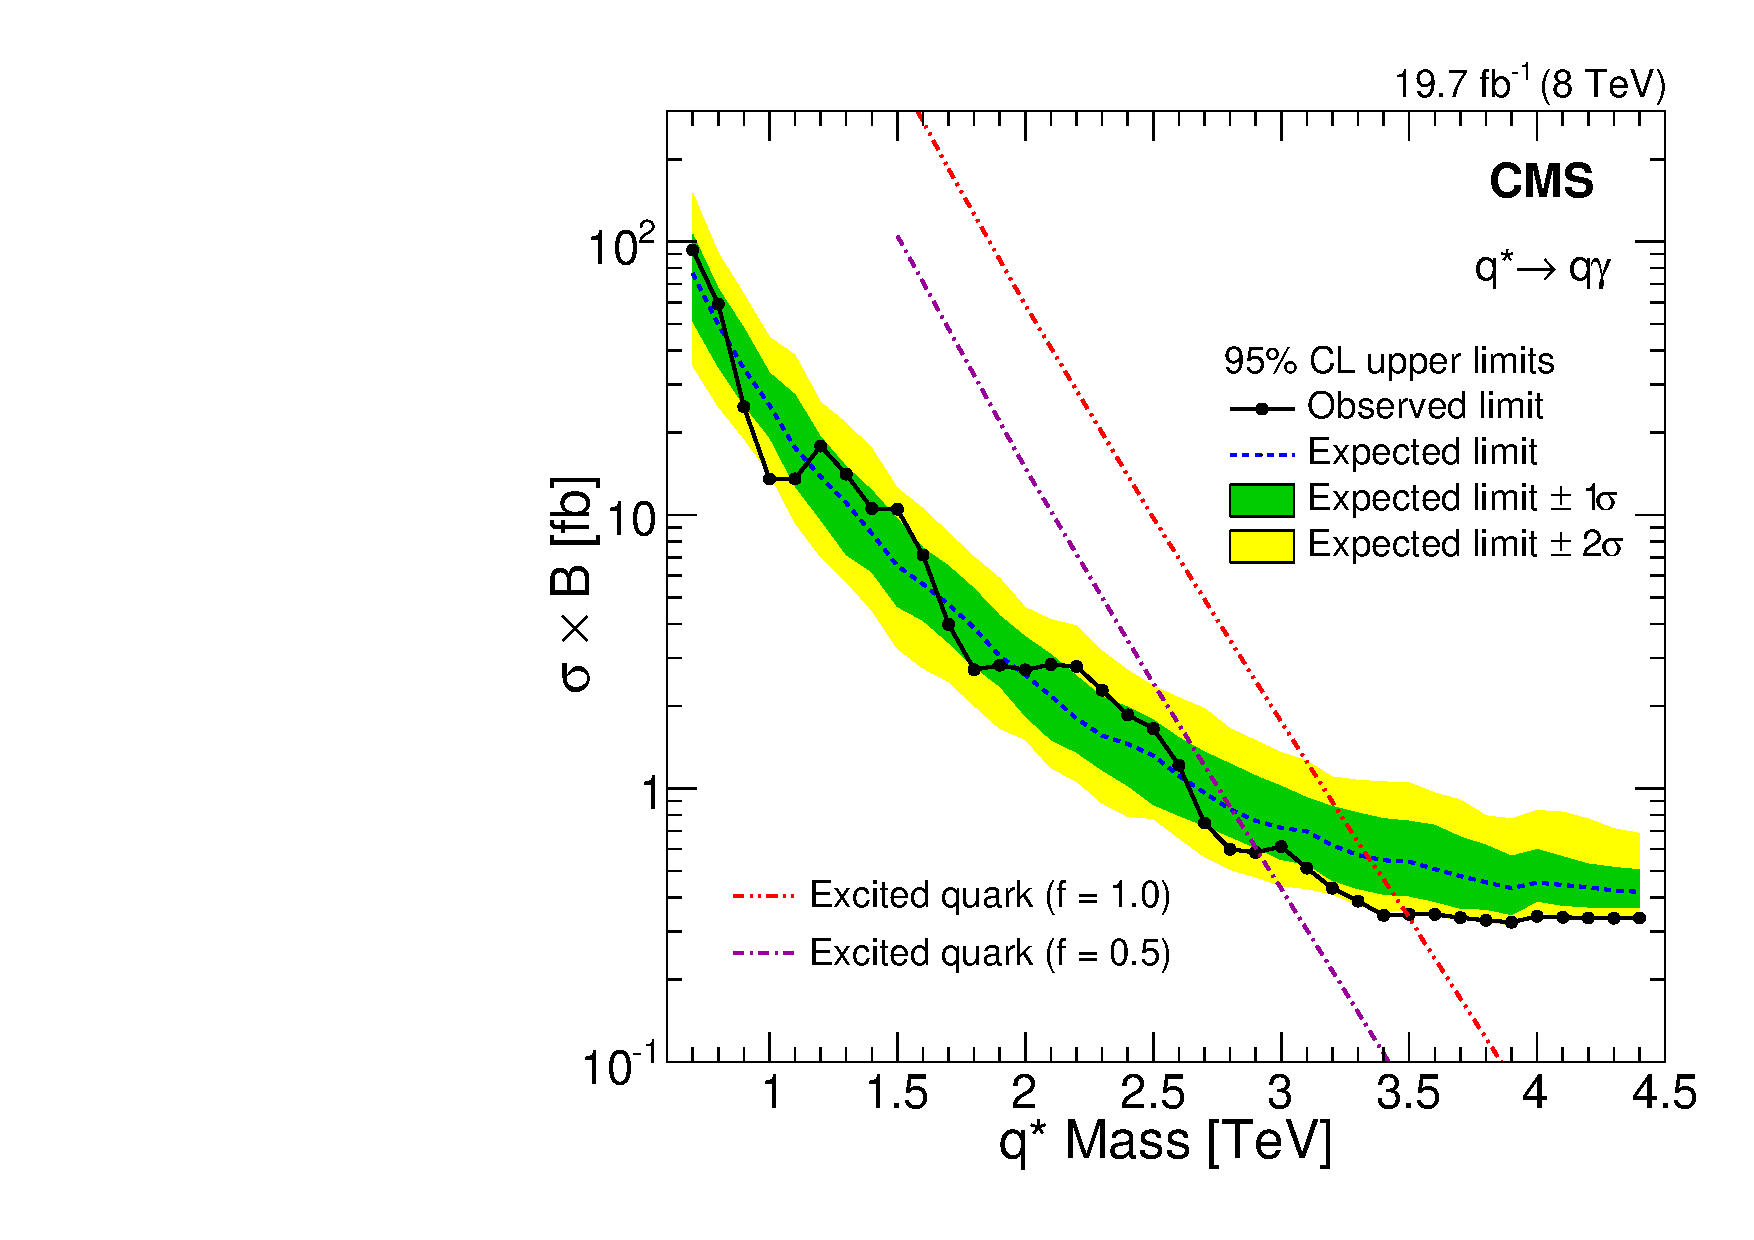
\includegraphics[width=10cm,height=8.5cm]{ch6/plots/ExcitedQuarksToGJ_fullfhalf_ObseExp_xs_Limits_paper_fb_v3.pdf} %% title size bigger
 \caption{The expected and observed 95\% CL upper limits on $\sigma\times\mathcal{B}$ for $\qstar\to\gamjet$ production, and comparison with 
          theoretical predictions for coupling parameters $f=0.5$ and $f=1.0$ respectively. The uncertainty at $1\sigma$ and $2\sigma$ levels 
          are shown as green and yellow bands, around the expected limits.  }
 \label{fig:LimitsfullHalf}
\end{figure}

\section{Summary}
This thesis presents a search for excited quarks in the \gamjet final state using 19.7\fbinv of proton-proton collision data at $\sqrt{s}=8\unit{TeV}$
at the CMS experiment. The data are found to be consistent with the standard model predictions and upper limits are placed on the $\sigma\times\mathcal{B}$
for \qstar predictions in the \gamjet final state. The experimental techniques used in this analysis can be summarized as follows:
\begin{figure}[h!]
\centering
% 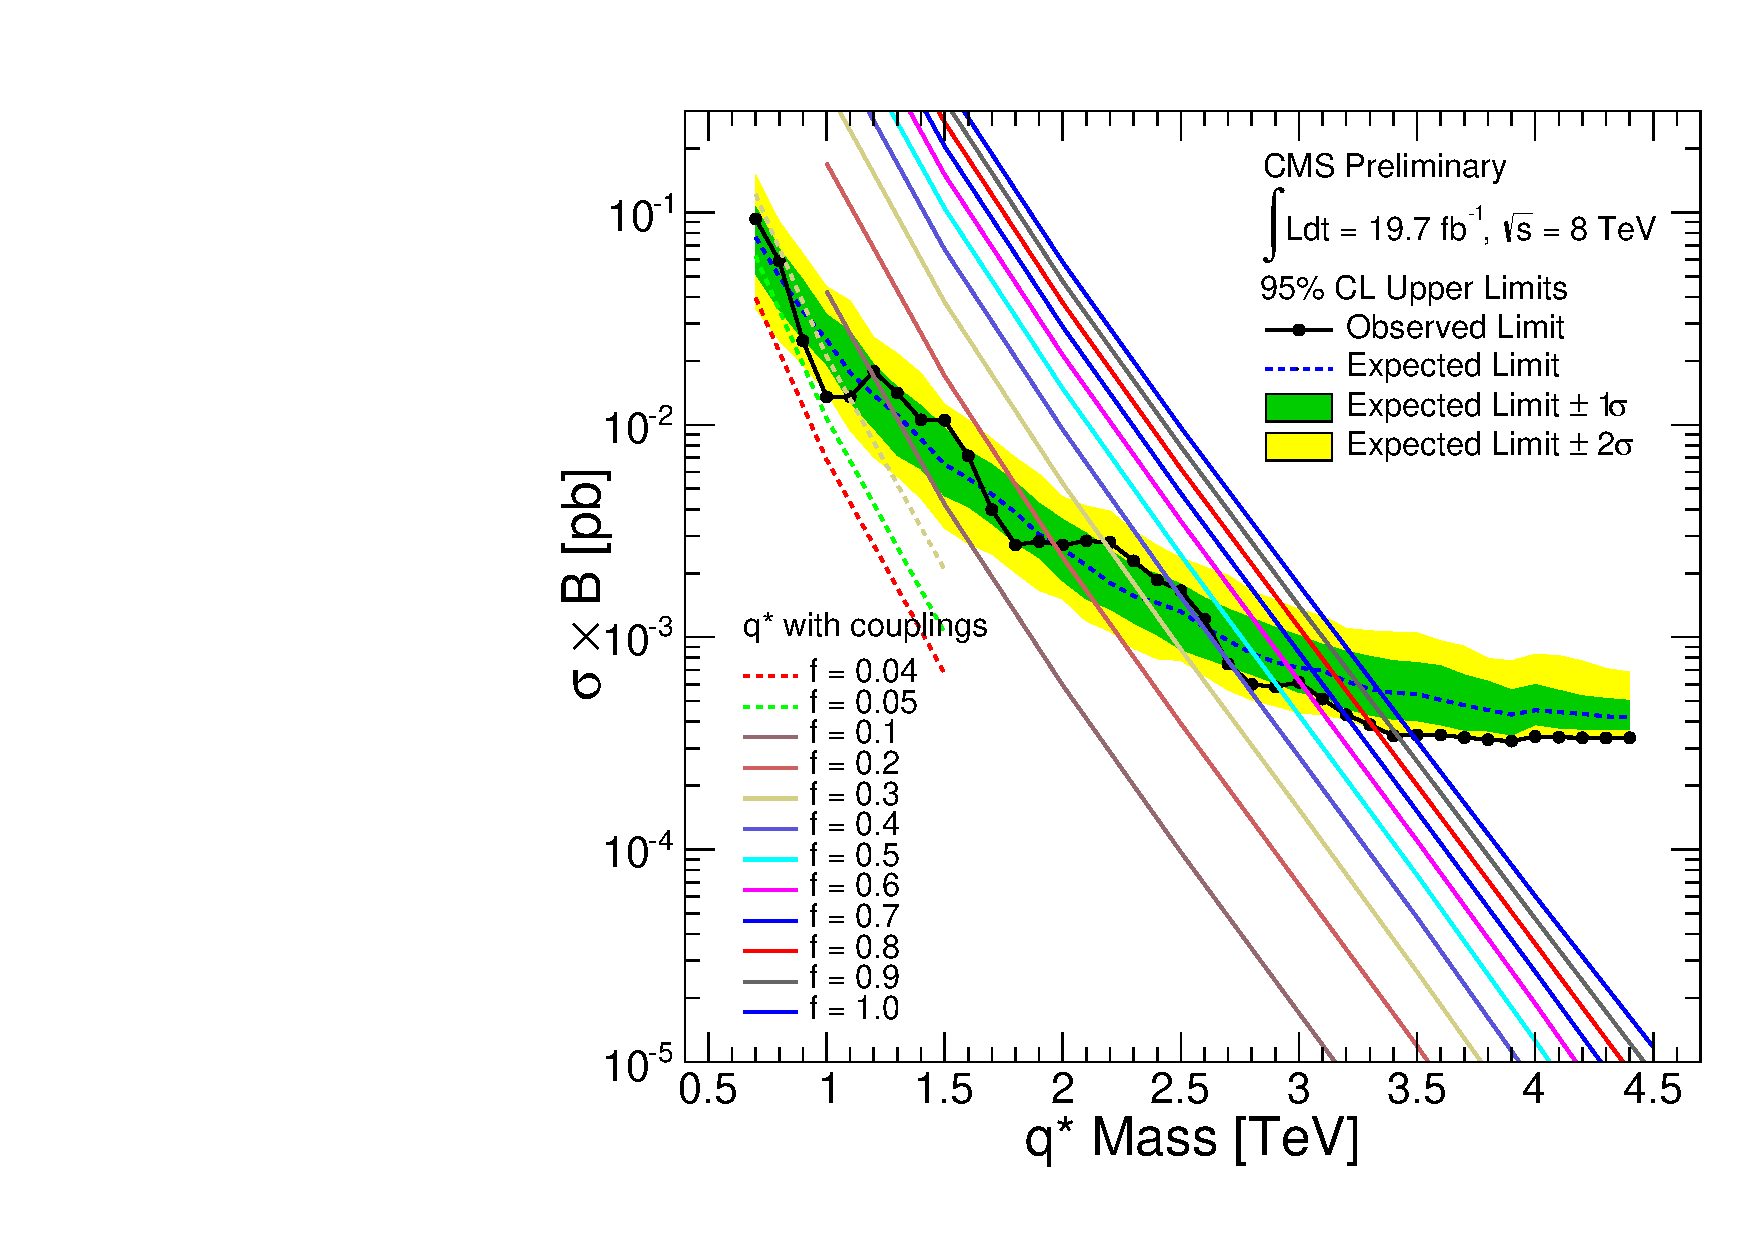
\includegraphics[width=12cm,height=10cm]{ch6/plots/ExcitedQuarksToGJ_AllCouplings_ObseExp_xsAccEff_Limits.pdf}
 %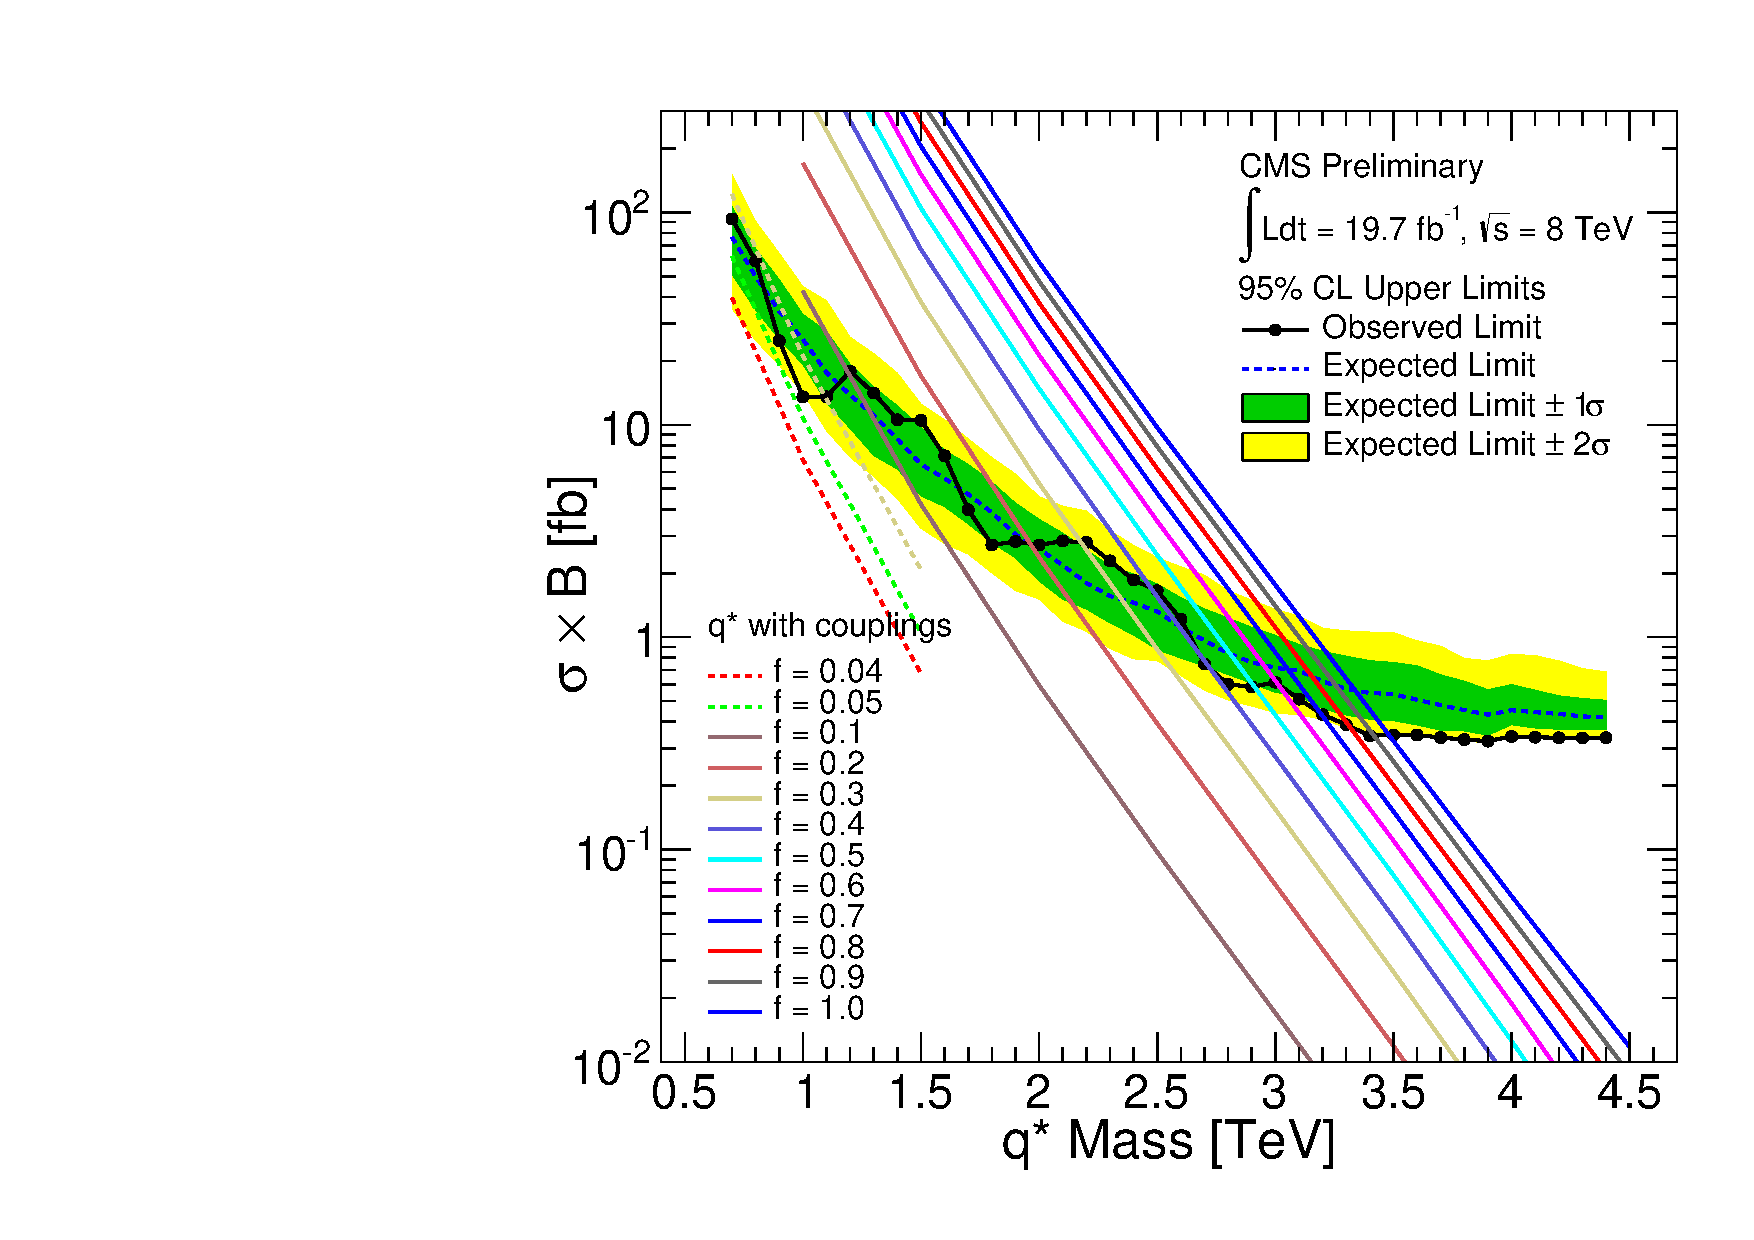
\includegraphics[width=12cm,height=10cm]{ch6/plots/ExcitedQuarksToGJ_AllCouplings_ObseExp_xsAccEff_Limits_fb.pdf}
 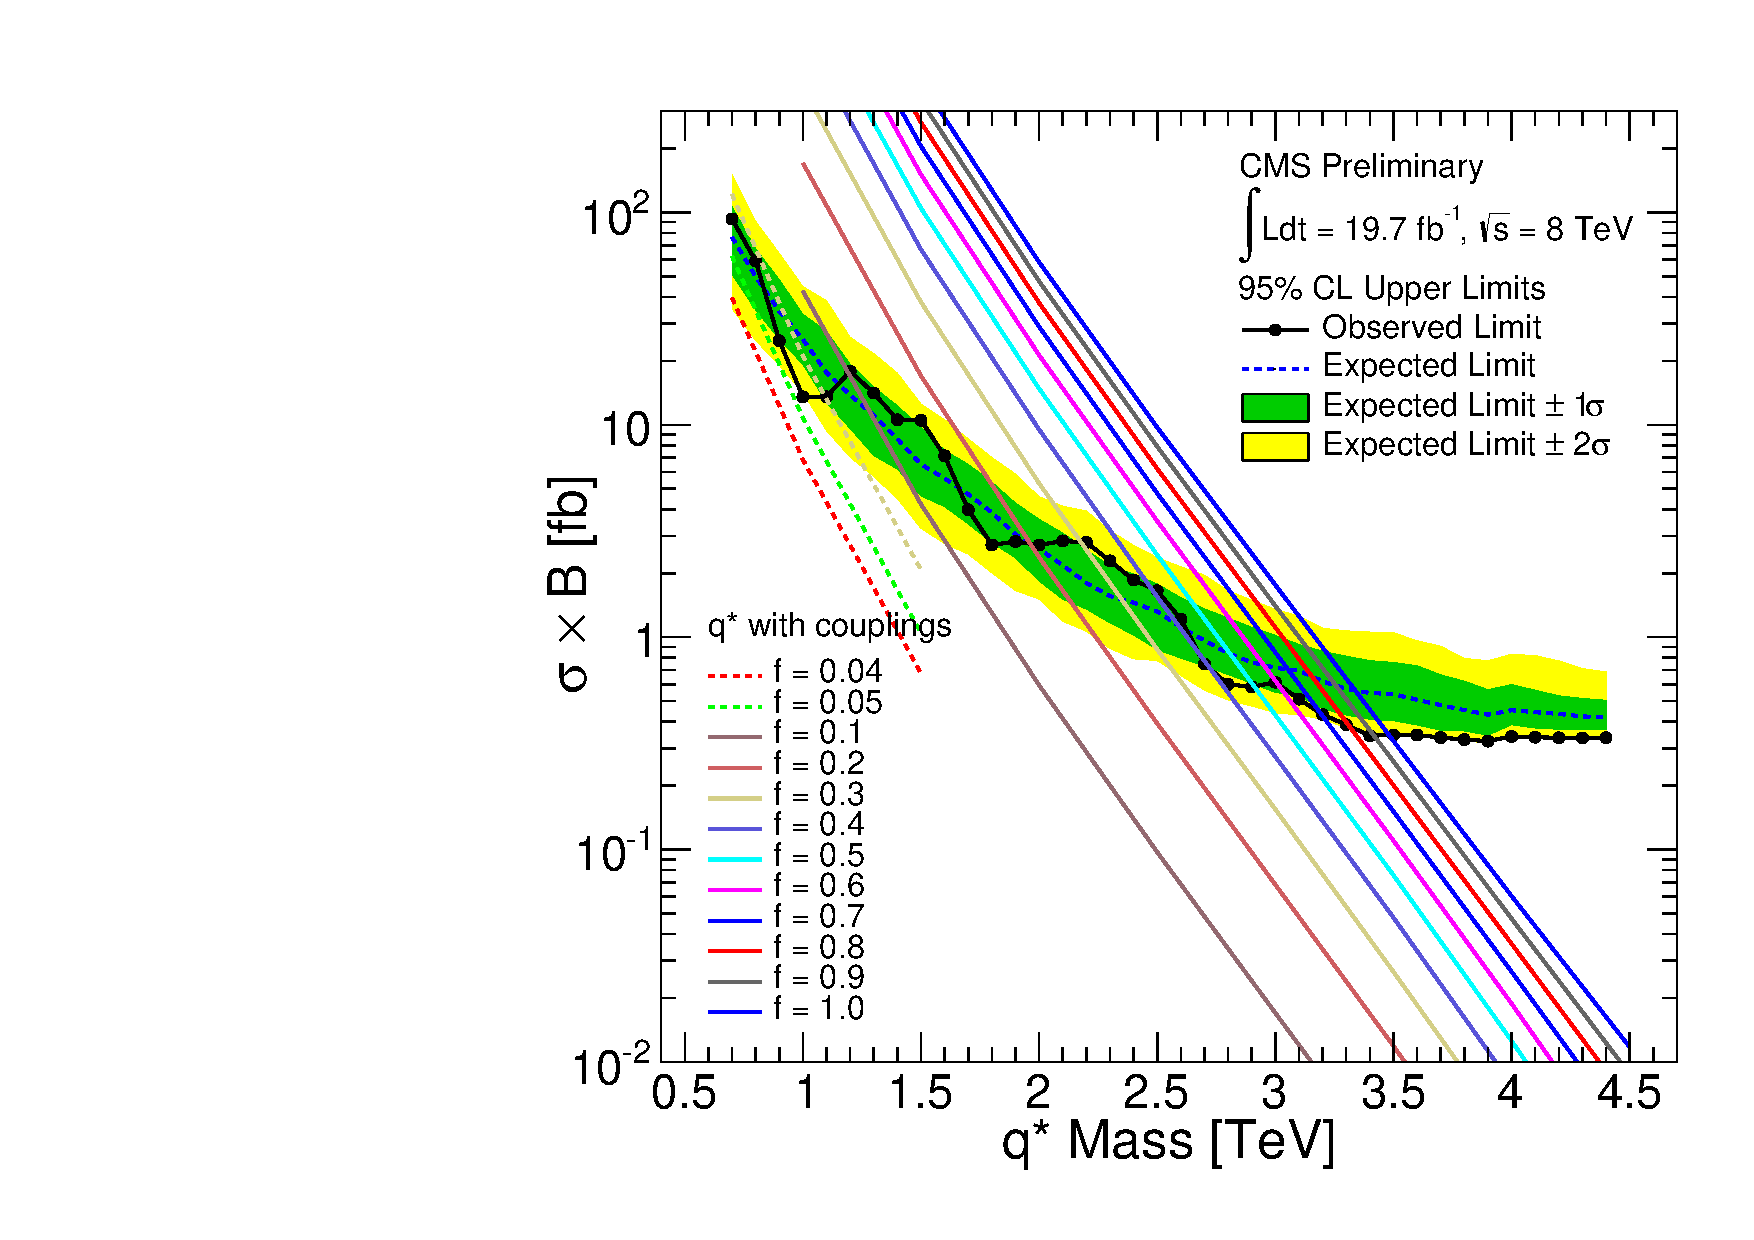
\includegraphics[width=10cm,height=8.5cm]{ch6/plots/ExcitedQuarksToGJ_AllCouplings_ObseExp_xsAccEff_Limits_fb.pdf}
 \caption{The expected and observed 95\% CL upper limits on $\sigma\times\mathcal{B}$ of excited quarks for coupling parameter $f$, ranging from 
          $f=0.004$ to $1.0$.}
 \label{fig:LimitAllCouplings}
\end{figure}
\begin{itemize}
\item Measure the \gamjet invariant mass spectrum.
\item Compare the measured invariant mass spectrum to simulated standard model Monte Carlo predictions. 
\item Fit the measured \gamjet invariant mass spectrum with a smooth parametrization and search for a resonant signal. 
\item If there is no evidence for the \gamjet resonance, evaluate model independent cross section upper limits and compare with the theoretical 
cross section prediction of the excited quark model.
\item Set the exclusion mass limits for the excited quark model. 
\end{itemize}
\begin{figure}[h!]
\centering
 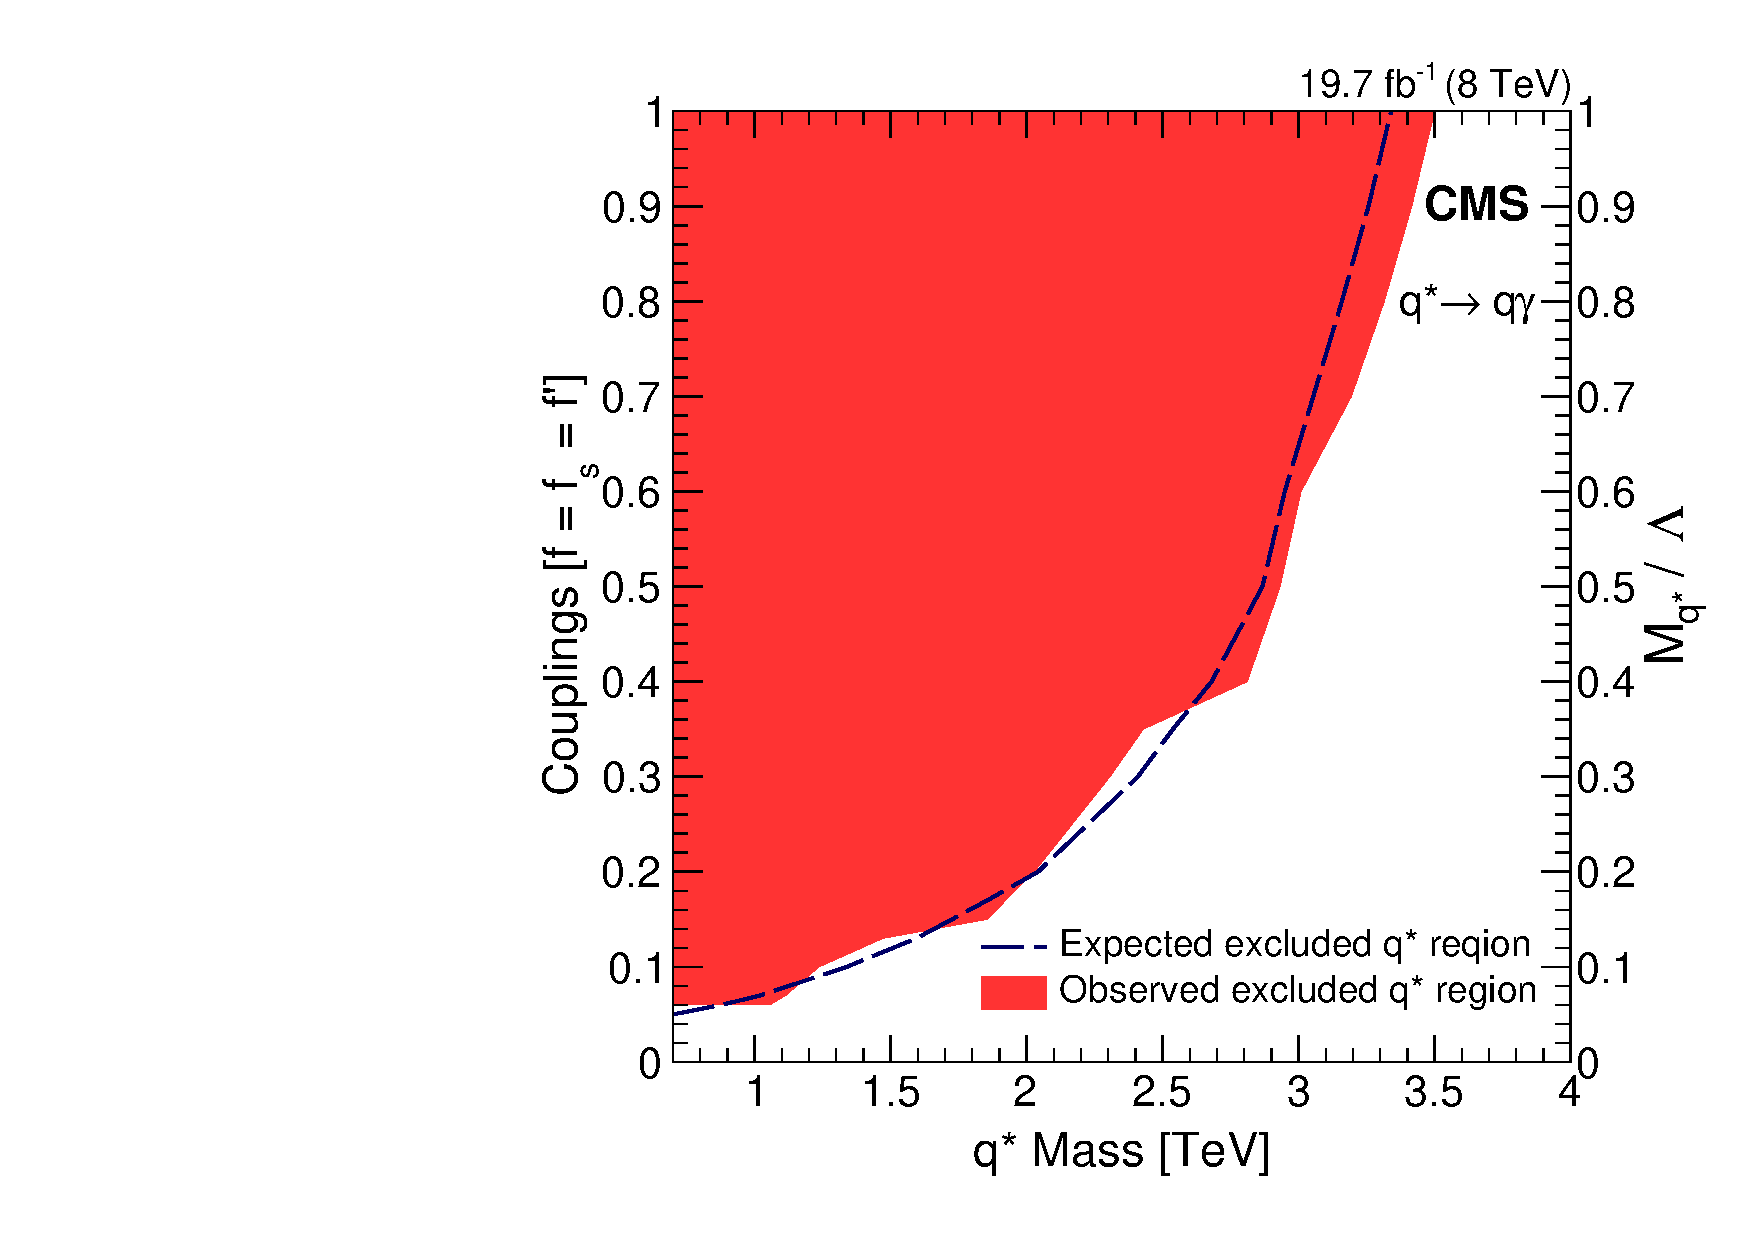
\includegraphics[width=10cm,height=8.5cm]{ch6/plots/CouplingvsMass_paper_FR.pdf}
 \caption{ The expected (dashed) and observed (red filled) excluded regions at 95\% CL as a function of \qstar mass and coupling strength
for $\Lambda=\mqstar$ (left axis) or the $\mqstar/\Lambda$ for coupling strength $f=1$ (right axis).}
 \label{fig:LimitMassCoupling}
\end{figure}
Comparing the cross section upper limits with the theoretical predictions, excited quarks with masses in the range, $0.7<\mqstar<3.5\unit{TeV}$
are excluded at 95\% confidence level limit under the assumption $f=1.0$. 

For the first time at the LHC experiment, the sensitivity of the excited quark search has also been investigated for coupling strength less than 
unity, as illustrated in \fig{\ref{fig:LimitMassCoupling}}. Excited quark masses in the range $0.7<\mqstar<2.9\unit{TeV}$ are excluded for
$f=0.5$. Furthermore, excited quarks with masses in the range $0.7<\mqstar<1.0\unit{TeV}$ are excluded for coupling value $f$ as low as $f=0.06$.

The work presented in this thesis has been published in Physics Letters B 738 (2014) 274-293.

